\chapter{5. Hardware Design and Analysis}

The vision of learnAir is to create a high-quality, affordable, and portable air quality monitor that (1) measures several pollutants, (2) measures ambient conditions like temperature, humidity, and light level, and (3) connects to a smartphone application that can display results, can send timestamp and geotagged data to the cloud, and can receive and display a prediction of measurement certainy based on machine learning applied to the data in the cloud.

Three learnAir devices have been built and tested.  The first (learnAir V1) is not portable, internet-connected, or battery powered-- it was solely used to collect sensor data that could be compared against higher quality MassDEP data for testing the feasibility and usefulness of predictive machine learning techniques.  This device was installed on a MassDEP (Department of Environmental Protection) monitoring site for 59 days-- from April 15th to June 13th 2016.

The second and third devices were designed to take the information gleaned from learnAir V1 and put it in a cheap, portable, smart-phone connected package.  The main circuit boards for LearnAir V2 and V3 were designed to match the size of the AlphaSense Analog Front End conditioning board-- a reasonably priced production board with three electrochemical gas sensors that has gained a strong reputation in the pollution sensing community.  These boards are BLE-enabled, and connect to two custom daughter boards for monitoring temperature, humidity, light level, UV exposure, and 3-axis wind speed.   

The two boards share power circuitry and most peripherals-- their central distinction is the main microcontroller.  LearnAir V2 is a fully functioning board based on the Atmel ATmega32u4, which requires an external RTC (real-time clock).  Firmware was written using a modified version of the Arduino codebase.  The third version is based on the STM32L152-- a more sophisticated, production-level microprocessor, with more optimization for low-power states, more SD card read/write support features, and an onboard RTC.  This third revision was also designed with a significantly smaller, soon-to-be available MEMS pressure sensor, which could reduce the volume occupied by the wind sensing module 50-fold (a large space savings from the current, large volume of 20mm x 60mm x 22mm).
     
The boards connect to a cross-platform smartphone application written in Javascript using Phonegap, a library that will compile javascript as webviews into iOS and Andriod applications.  It has plugins to access the phone GPS, and a simple D3.js library was used for plotting.  ChainAPI- our backend solution- supports  websocket connections and a subscription model to push data to the cloud and receive the latest predictions.



\section{LearnAir Version 1}
\FloatBarrier

LearnAir V1 was created to collect data with a variety of cheaper air quality sensors at a MassDEP monitoring site, to test our ability to predict a sensor's accuracy with machine learning by comparing it to a high quality reference.  The final box is 200mm x 120mm x 75mm (~ 8 x 5 x 3in), and houses two main subsystems.

\begin{marginfigure}
 	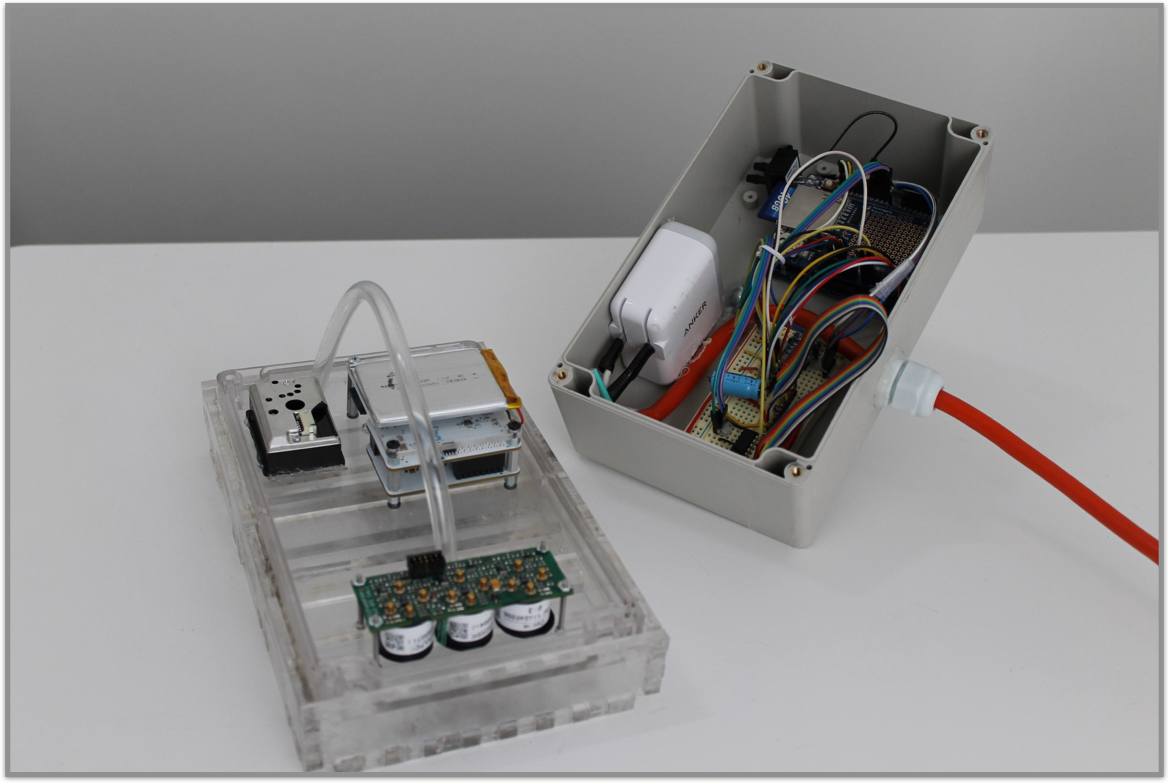
\includegraphics[width=\textwidth]{visuals/learnairV1}               
 	 \caption{LearnAir Sensor installed at MassDEP site, opened}
  	\label{fig:learnairv1}
\end{marginfigure}

\begin{figure}[htb]
 	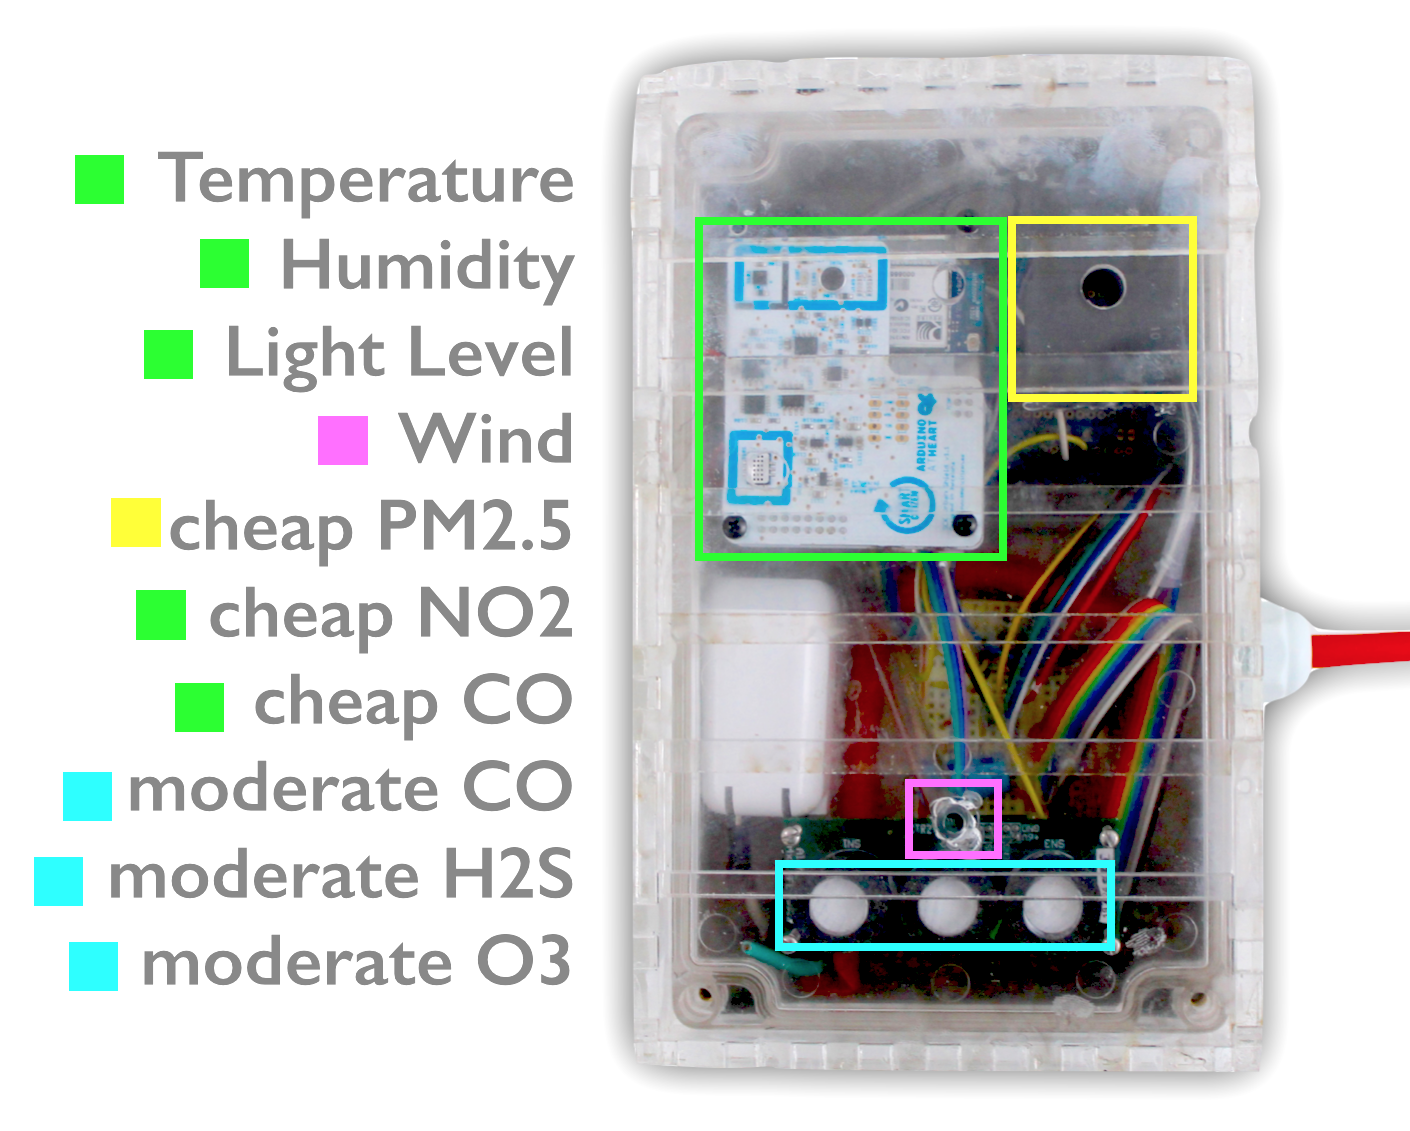
\includegraphics[width=\textwidth]{visuals/learnairV1_labeled}               
 	 \caption{LearnAir Sensor installed at MassDEP site}
  	\label{fig:learnairv1_labeled}
\end{figure}

The first sub-system is an off-the-shelf air quality monitoring system called the SmartCitizen Kit (frequently abbreviated SCK). \cite{sck}  The SmartCitizen Kit is Arduino-based (using the ATmega32u4), so custom code can easily be written and applied to the hardware.  This system was used in an offline data-logging mode, with raw data streams stored to the onboard micro-SD card for later retrieval.  

The SmartCitizen Kit includes several important sensors for our machine learning test.  It has a \textbf{DS1307} real-time clock for timestamping data and sample timing, a \textbf{MicroSD slot} for saving CSV files, a ROHM \textbf{BH1730FVC} I2C light sensor to monitor ambient light levels, a PUI \textbf{POM-3044P-R} electret microphone for monitoring ambient noise level, and a Sensirion \textbf{SHT21} I2C temperature and humidity sensor.  Most importantly, it has an E2V \textbf{MiCS-4514} CO and NO2 sensor.  This is a \$10, MEMS sensor-- one of the cheapest air quality sensors available.  It works on a Reduction/Oxidation principle, and has small internal heating elements.  It claims a 1-1000 ppm measurement range for CO and a 0.05-10ppm measurement range for NO2, and omits any information about reaction speed or cross-sensitivity in the datasheet.

The SmartCitizen Kit was mounted to the front of the case, with a small hole to expose the relevant sensors to the air.  Every hole in the case was gasketed with silicone, and the front of the case was mounted face down to minimize rain exposure.  Furthermore, a clear-acrylic, overlapping, slotted cover was designed to further protect the exposed sensing elements from rain and direct exposure.  

Despite the effort to protect the circuitry, the SmartCitizen Kit corroded severely in our first outdoor test.  A new kit was installed, this time with a layer of conformal coating added to prevent corrosion (Figure \ref{fig:sck_corroded}).  This addition prevented further corrosion for the remainder of the two month installation.    

\begin{marginfigure}
 	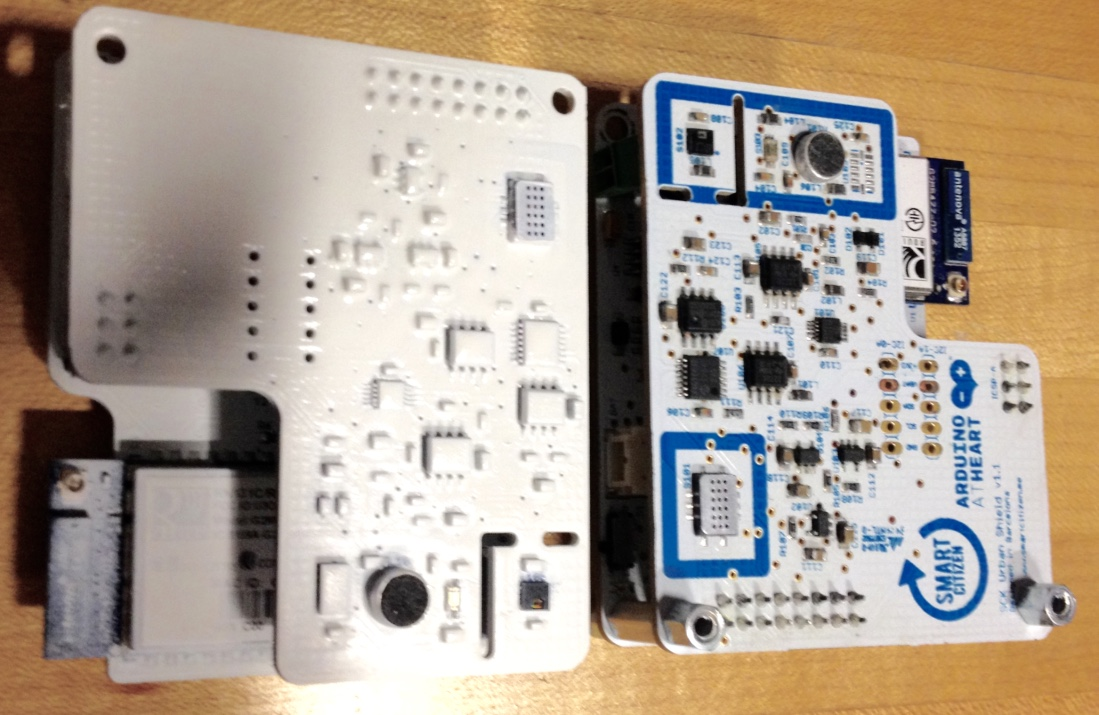
\includegraphics[width=\textwidth]{visuals/sck_conformal}               
 	 \caption{Corroded SmartCitizen Kit on the right, Conformal-coated new kit on the left.  Relevant sensors on the new kit were taped off before coating to prevent contamination}
  	\label{fig:sck_corroded}
\end{marginfigure}

Besides the SmartCitizen Kit, a custom Arduino-based sub-system is part of the platform.  This system is based on an Arduino Leonardo board (Atmel ATmega32u4) with an Adafruit data-logging shield (which includes an \textbf{SD card slot} and a Maxim \textbf{DS1307} RTC for timestamping-- the same RTC as the SmartCitizen). 

Three main sensor sub-systems were connected to this Arduino using a secondary prototyping board.  First, a \$10 Sharp \textbf{GP2Y1010AU0F} Optical Dust sensor was connected.  This sensor requires an external charging circuit to store energy for a narrow IR light pulse that is used to detect scattering.  These sensors have a reasonable reputation, and have shown good correlation with better quality sensors under controlled conditions indoors.  \cite{prabakar2015, austin2015} In real-world situations, they are unreliable.  

Secondly, an \textbf{AlphaSense Analog Front End Board} was connected.  This board supports three AlphaSense electrochemical gas sensors, which each have a Working and Auxiliary Electrode measurement.  Additionally, this board provides an onboard temperature measurement for sensor calibration.  All of these signals were multiplexed through an external TI \textbf{CD54HC4051e} multiplexer before connection to the Arduino 10-bit ADC.  Alphasense sensors are well-reputed, mid-level sensors-- they typically cost \$60-100 each, with the support circuit adding an additional \$150 in cost.  These sensors have t$_9_0$ response times of 10 ppm in ~20 seconds for CO, 1 ppm in ~30 seconds for NO2, and 100 ppb in ~15 seconds for O3.  Cross-sensitivity of the O3 sensors to NO2 is quite high (70-120\% measured with NO2 levels of 5ppm), as well as vice versa. (The NO2 sensor picks up 30-60\% of O3 at 100ppm.)  Other cross-sensitivities are well-documented and much smaller.  These sensors sport very low monitoring thresholds, well-characterized calibrations for electrolyte depletion and temperature dependence, and specified operating ranges for pressure, temperature, and humidity.

Finally, an Omron \textbf{D6F-PH} differential pressure sensor was included as a cheap, experimental way to measure airflow and wind.  This pressure sensor has two outlets- one was left vented into the box, and one was connected through a tube to the surface of the device.  Airflow over the top of the device creates a measurable pressure differential.  This sensor runs an I2C interface at 3.3V (which is incompatible with the 5V Arduino), so an external BSS138 level shifter from Adafruit was required to properly interface with the sensor.  All of these sensors were mounted to the front of the case, and gasketed to prevent unintended air exposure.

The final system is shown in Figures \ref{fig:learnairv1} and \ref{fig:learnairv1_labeled}.  An extension cord was spliced and soldered to a dual port USB charger, with powered both systems off of 5V USB.  This extension cord was inserted through a cable gland in the side of the box.  A metal mounting bracket extends from the back of the device.  Both sub-systems were configured to sample their sensors every 30 seconds.




\section{MassDEP Site}

Thanks to the generosity of the Massachusetts Department of Environmental Protection, I was given full access to their Roxbury Monitoring Site, allowed to co-locate the learnAir V1 sensor with their sensing inlet (approximately 3 feet away), and provided (normally unpublished) high time-resolution data.  The Roxbury monitoring site is the only one in the greater Boston area that has the capability to monitor particulate levels (through hourly Beta Attenuation Monitoring [BAM] measurements of black carbon), as well as minute-resolution data for trace gases (CO, NO, NO2, and O3).  We were also provided with high quality, minute-resolved windspeed and wind direction data, which we used to analyze our experimental differential pressure wind sensor and included as a training feature in our machine learning data.      

\begin{marginfigure}[3.5cm]
 	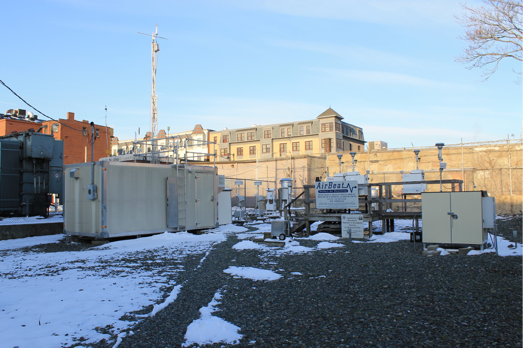
\includegraphics[width=\textwidth]{visuals/epa}               
 	 \caption{A picture of the Roxbury MassDEP measurement site where the LearnAir sensor was installed}
  	\label{fig:epa}
\end{marginfigure}

\begin{figure}[htb]
 	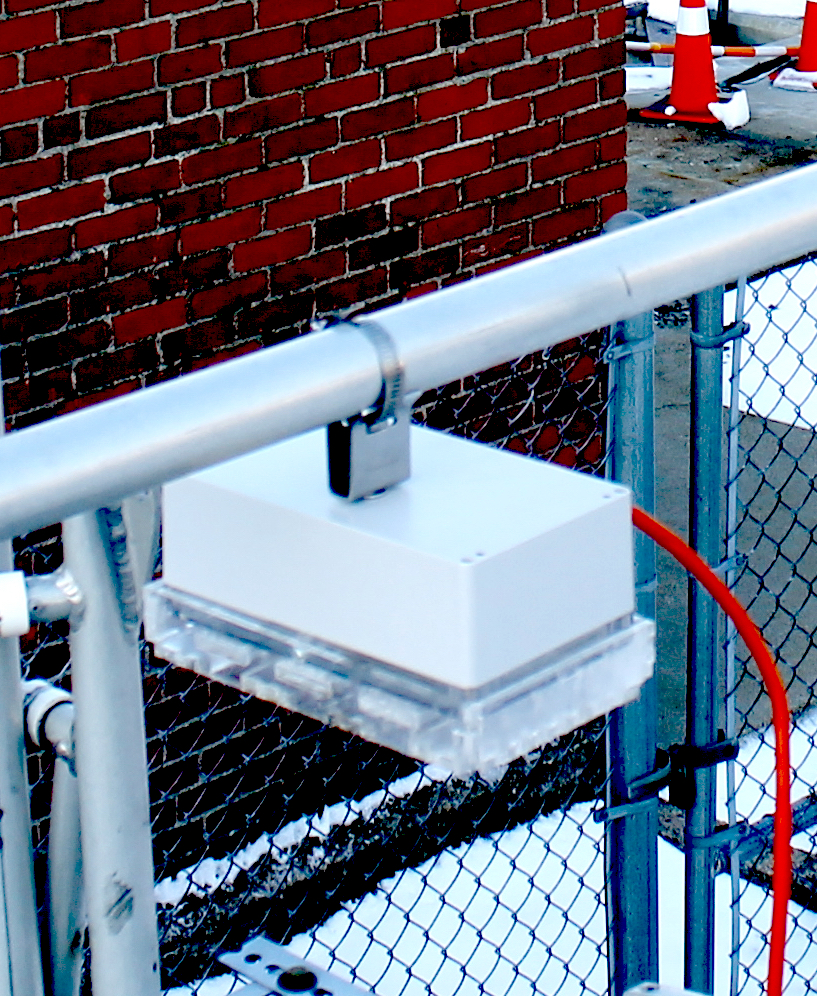
\includegraphics[width=\textwidth]{visuals/learnairV1_installed_zoomed}               
 	 \caption{LearnAir Sensor installed at the MassDEP site, close-up}
  	\label{fig:learnair_installed_zoomed}
\end{figure}

\begin{figure}[htb]
 	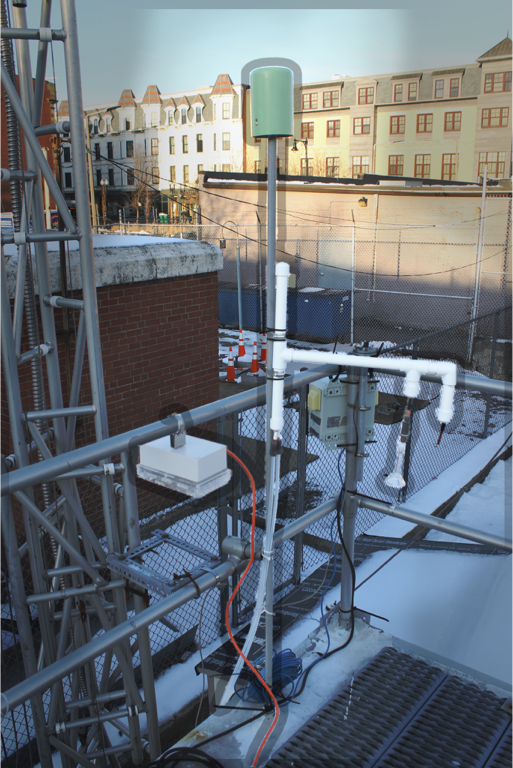
\includegraphics[width=\textwidth]{visuals/epa_zoom}               
 	 \caption{LearnAir Sensor (box on left) installation next to MassDEP inlet (top of pole on right)}
  	\label{fig:epa_zoom}
\end{figure}

The data provided by MassDEP is monitored weekly for quality assurance.  Each piece of sensor technology is in the \$10-100k range.  The EPA specifies Federal Reference Method (FRM) devices (devices that are accepted as the reliable standard for research use and to compare other devices against), as well as Federal Equivalence Method (FEM) devices, which may use other techniques but are acceptable replacements for FRM techniques.  All of these reference devices include FRM or FEM certification.

Black Carbon measurements were done with a Teledyne Model 633 Aethalometer sensor system which operates similar to the BAM style measurement.  This type of measurement draws air through filter paper for a period of time, and then irradiates it with UV and IR light to see how well the captured particulate attenuates it.  This means that-- though the measurement is incredibly robust and reliable-- the time-scale for measurements is on the order of an hour, and is an average of the accumulation over that period.  For the system we were using, a `10 a.m.' reading is exposed to air from 10:00 to 10:50 a.m., and measured between 10:50 and 11a.m., before the next reading begins.  Measurements are reported as \(\mu g/m^3\).
   
Wind speed and direction data was captured on a minute time-scale with a high-quality, vane style Met One 50.5H Sonic anemometer.  Trustworthy wind sensing data at these price points is non-controversial.  Measurements are reported in approach angle (degrees) for the direction and m/s for speed.

For gaseous pollution measurements, all of the reference equipment comes from Teledyne Advanced Pollutant Instruments.  The system is fed by an expensive, size-selective inlet with precise flow control.  Air is actively pulled through the system at a known, fixed rate.   Cross-sensitivity is not an issue for any of these devices.  

For NO and NO2 measurements, the Teledyne Model 200E Chemiluminescence Sensor is used. NO is measured by exposing the gas to O3 and measuring chemiluminescence, and a catalytic-reactive converter then converts NO2 to NO and repeats the measurement.  It has a precision of 0.5\% of its reading, and a t$_9_5$ of 60 seconds for its full operating range of 20 ppm, at a 0.5 L/min flow rate.  It is capable of reporting the average over a sample period or the instantaneous value.  It includes an adaptive filter that averages 42 samples over 5.6 minutes by default, unless it detects a rapid change in concentration (comparing an instantaneous reading to the long filter average), in which case it switches to a short-term, 6 sample, 48 second average.     

For O3 measurements, the FEM Model T400 UV Absorption system is used.  It has a 0.5 ppb sensitivity, and a t$_9_5$ of 20 seconds for its full operating range of 10ppm at a 800cc/min flow rate.  This system works on the Beer-Lambert law, alternately comparing the absorption of a stream the sampled air with an O3 filtered stream every 3 seconds using UV light (and correcting for temperature and pressure of the gas).  It is capable of reporting the average over a sample period or the instantaneous value. Its adaptive filter averages 32 samples over 96 seconds by default, switching to a short-term, 6 sample, 18 second average with rapid changes in concentration.

For CO, the FEM Model 300EU Gas Filter Correlation system is used.  It has a 0.5\% precision, and a t$_9_5$ of 30 seconds for its full operating range of 100ppm, at a 1.8 L/min flow rate  It similarly uses the Beer-Lambert law and IR light to compare a scrubbed sample with the untouched air.  It is also capable of reporting the average over a sample period or the instantaneous value.  Its adaptive filter averages 750 samples over 150 seconds by default, switching to a short-term, 48 sample, 10 second average with rapid changes in concentration.     

We installed the learnAir system face-down on the roof railing of the main air monitoring building, about three feet from the reference sensor inlet, as seen in Figure \ref{fig:epa_zoom}.  Our sensor and the inlet both face downward, however the Federal reference system has active airflow.  These inlets are mounted approximately 12 feet in the air and about 30-40 feet from the street.

\FloatBarrier
\begin{figure}[htb]
 	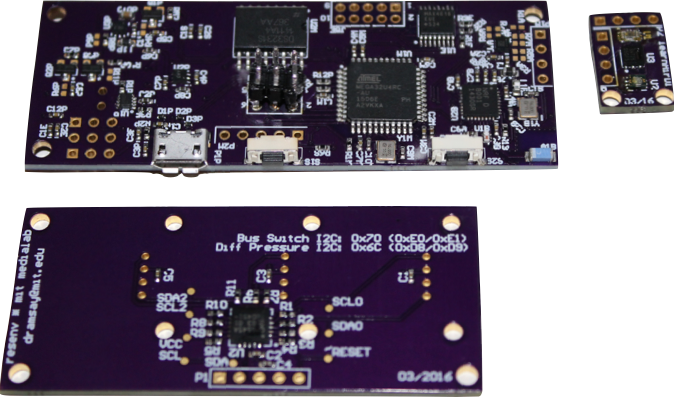
\includegraphics[width=\textwidth]{visuals/learnairV2_out}               
 	 \caption{Main and daughter boards of learnAir V2.0}
  	\label{fig:learnairv2_out}
\end{figure}
\FloatBarrier
\section{LearnAir Version 2}
\FloatBarrier

While the first hardware device we built was designed to collect data for testing and validation of learning algorithms, it does not represent a scalable, portable, cheap solution.  For that, we designed learnAir V2.

LearnAir V2 was created to be inexpensive, handheld, and portable.  It is designed to measure ambient conditions-- just like learnAir V1-- while still collecting the relevant air quality data.  It is battery-powered and smartphone connected, so that data can be seamlessly GPS-tagged, viewed in real-time, and sent to the cloud.  The outline of the internal circuit board was designed to mate with the AlphaSense AFE board.  AlphaSense sensors come well recommended in the air quality sensing community.  

The circuit design for LearnAir V2 is shown in Figure \ref{fig:learnairv2_out}.  It consists of a main board, designed around the Atmel ATmega32u4, and two daughter boards.  The main board sports a \textbf{micro-SD card} slot for storing data, a Nordic \textbf{nrf8001} with a chip antennae for Bluetooth Low Energy communication with a phone, a \textbf{microUSB} connector for charging the device and interacting with the microcontroller over USB, a ST \textbf{LIS2DH12} accelerometer to measure 3-axis motion and vibration, a TI \textbf{MAX4618} multiplexer to handle communication and mating to the AlphaSense frontend board, a Maxim \textbf{DS3231} RTC (from the same family as the DS1307 used in learnAir V1 but with temperature compensation and much more accurate timing), and standard breakout headers for several I2C and SPI environmental sensing peripherals at both 5V and 3.3V.  The main circuit is powered off of 3.3V to save on power, but 5V power handling is included.  Power to 5V peripherals can be programmatically shut on and off by the microcontroller for power saving when sleeping high quiesent devices.  Schematics for learnAir V2 can be found in Appendix B.

\begin{marginfigure}[3.5cm]
 	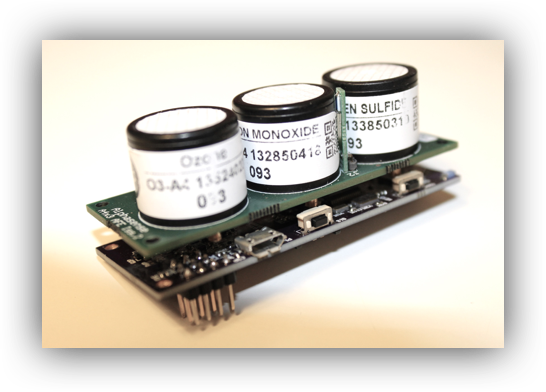
\includegraphics[width=\textwidth]{visuals/learnairV2}               
 	 \caption{Second revision, Atmel based learnAir main board mated with the AlphaSense sensor frontend}
  	\label{fig:learnairV2}
\end{marginfigure}

Two daughter boards were designed to connect with the main board learnAir board.  This modular design gives more flexibility for housing the device, simple upgradability, and separates concerns when testing/verifying the circuitry.  

The first of these daughter boards includes all sensors that need to be mounted on against the edge of the device, either in contact with the air or with direct access to sunlight.  This small board includes a ROHM \textbf{BH1730FVC} I2C light sensor, a Vishay \textbf{VEML6070} I2C UV sensor, and a Sensirion \textbf{SHT25} temperature and humidity sensor.  The SHT25 is similar to the SHT21 used in learnAir V1, but with slightly tighter tolerances. 

The second daughter board is designed to hold three Omron \textbf{D6F-PH} differential pressure sensors, for 3-axis wind sensing.  This is the same pressure sensor as was tested in the learnAir V1 device.  Since the D6F-PH does not come with selectable I2C addresses, this daughter board also has an NXP PCA9545	 I2C-bus switch to selective open the I2C bus between one of the three pressure sensors and the main learnAir board.  This I2C bus switch is itself addressable and controllable over I2C, so no extra pins are required to connect it.  Schematics for both daughter boards can be found in Appendix B.

Besides the connections to the three AlphaSense gas sensors controlled by the AlphaSense Analog Front End board, the main board is also equipped to connect to either a Sharp GP2Y1010AU0F (as tested in the learnAir V1 device) or the much more accurate \$500 AlphaSense \textbf{OPC-N2}.  The OPC-N2 takes advantage of Mie scattering algorithms and uses higher quality optics, but it is insensitive to particles under a few hundred nm and has a limited feature-set around flow filtering and control.  Independent validation of the OPC-N2 has been mixed, and the device includes a built in fan (demanding a lot of power for a portable device), but it offers an enticing combination of cost and size given its sophistication.

A final physical design of the learnAir V2 device was modeled in SolidWorks, and fits in the palm of a user's hand (Figure \ref{fig:learnairbox}).  The final cost of the OPC-N2 version is around \$1k, while the Sharp version is closer to \$600.  

\begin{figure}[htb]
 	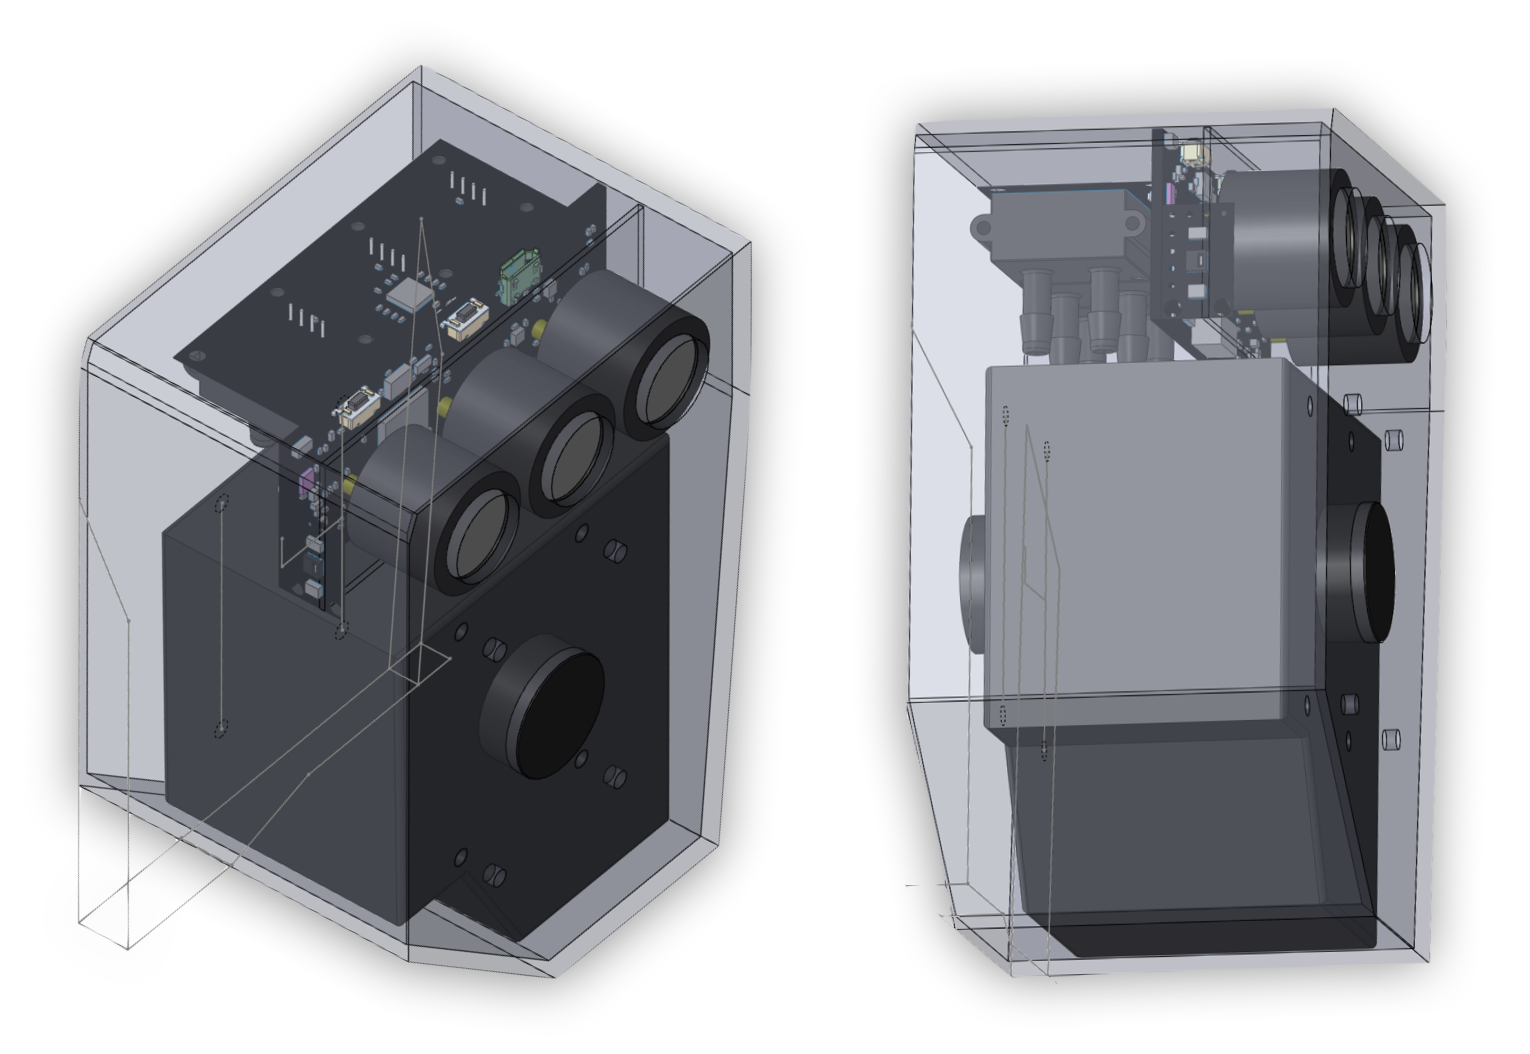
\includegraphics[width=\textwidth]{visuals/learnairV2box}               
 	 \caption{Final design of the portable system}
  	\label{fig:learnairbox}
\end{figure}

Once the hardware was actually designed and built, firmware to control the device needed to be created.  The Arduino environment and libraries were used to write code for learnAir V2.  Since this is a demanding application, the standard pinouts used by typical Arduino boards needed to be redefined.  LearnAir clocking and custom pin mapping definition files were added to the Arduino environment-- now, similar to `Leonardo' and `Due' and other boards, the `learnAir' board can be chosen and programmed as an option from the Arduino environment dropdown menu.  Firmware and board definition code is available in Appendix B.  The completed code and hardware was tested with a learnAir smartphone application and shown to work reliably.

\FloatBarrier

\begin{figure}[htb]
 	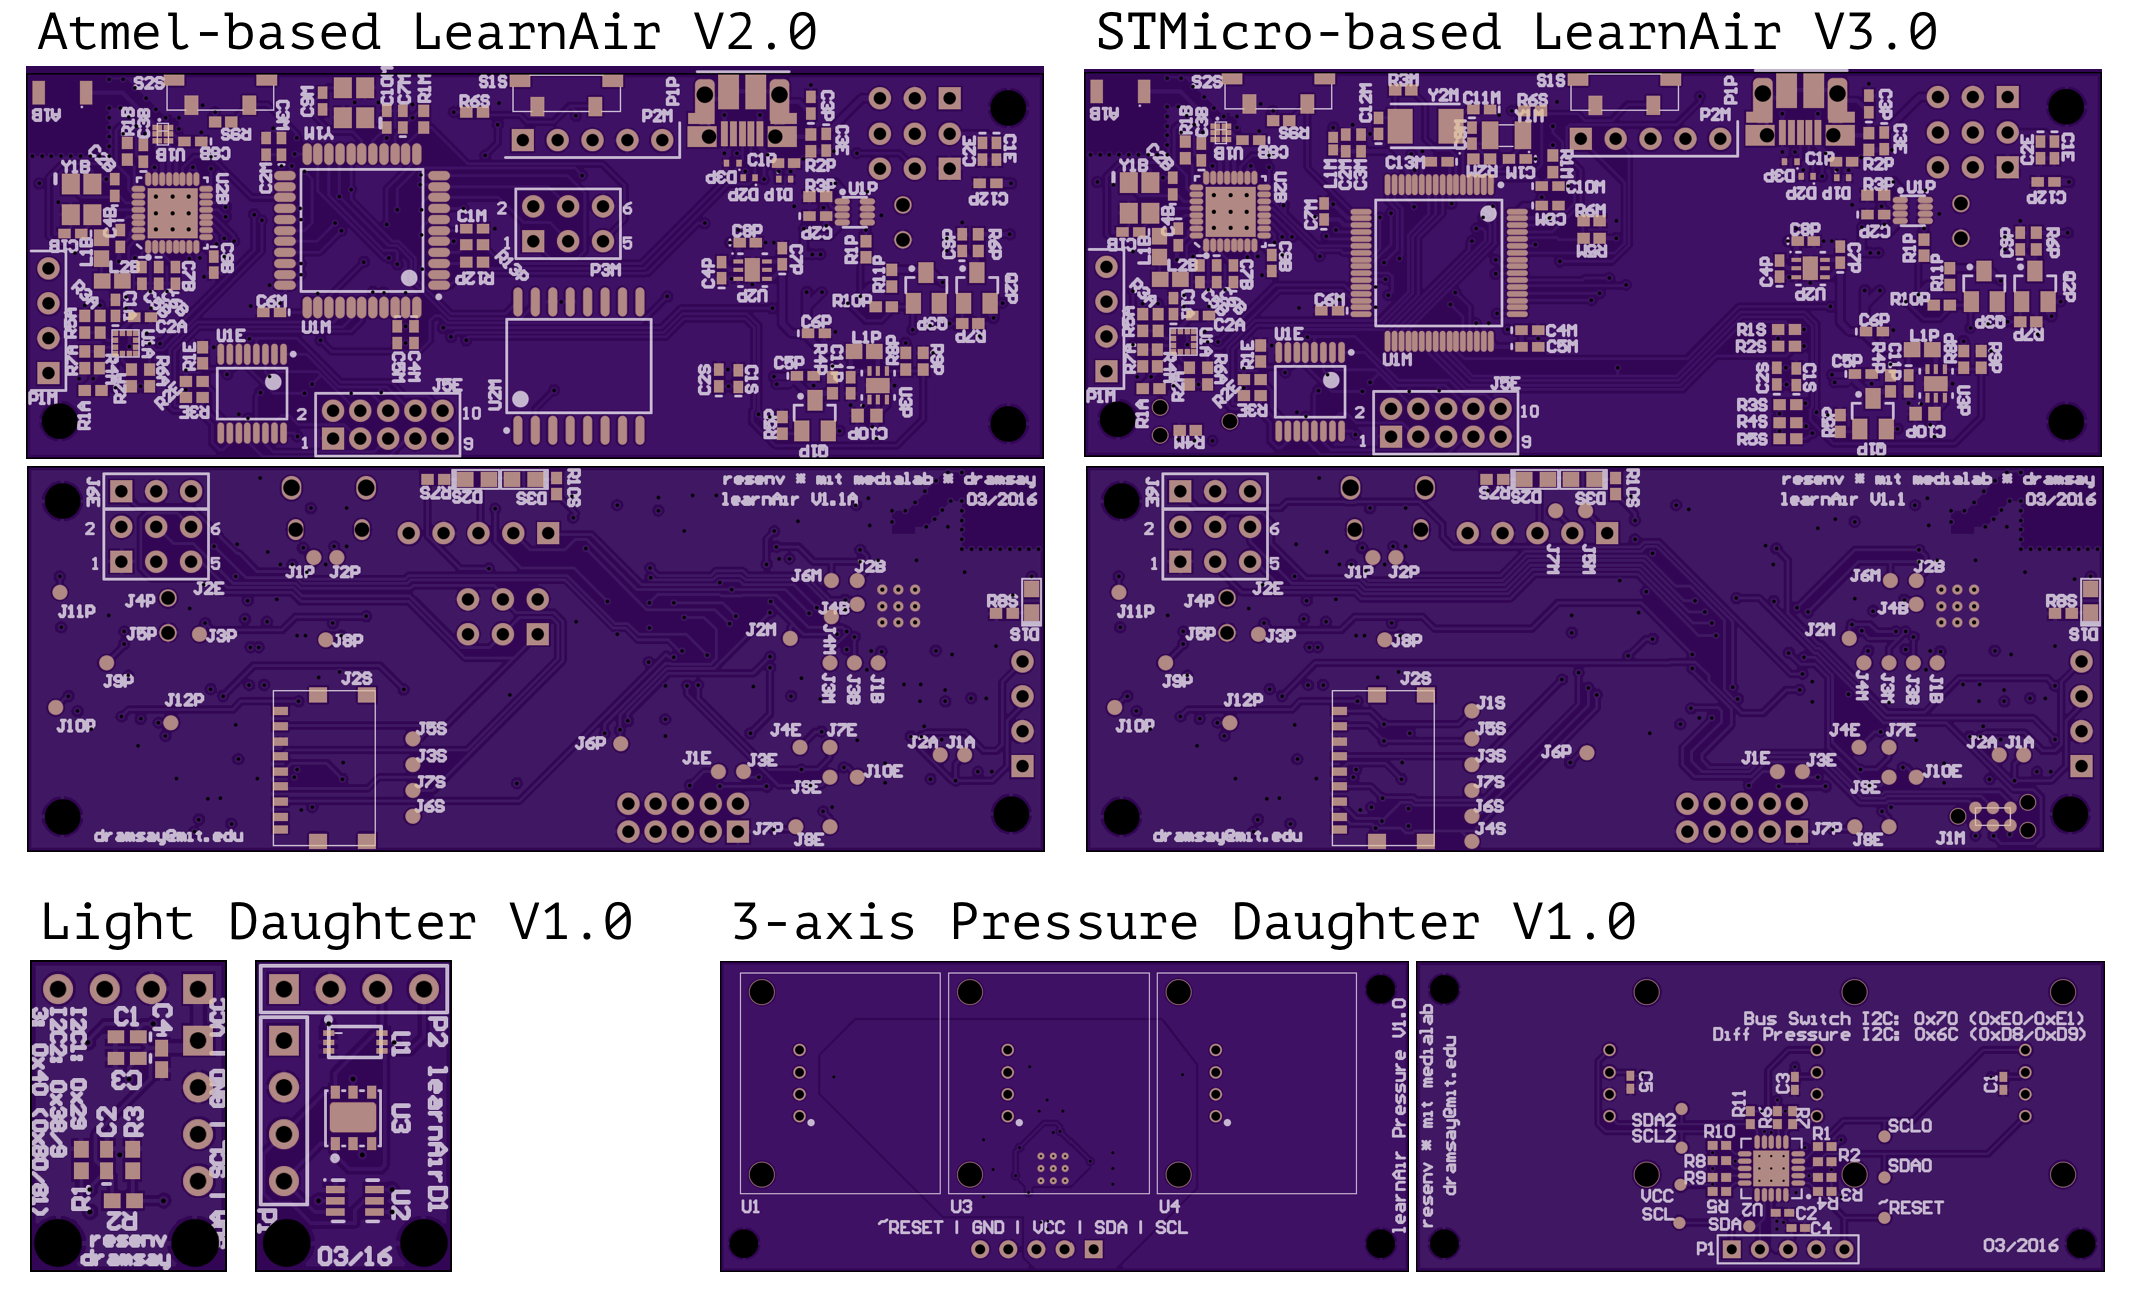
\includegraphics[width=\textwidth]{visuals/layouts}               
 	 \caption{Layouts for revisions 2.0 and 3.0 of the learnAir board}
  	\label{fig:layouts}
\end{figure}


\FloatBarrier
\section{LearnAir Version 3}
\FloatBarrier

The third version of learnAir hardware is very similar to the second in most ways.  It supports the same daughter boards, peripherals, power circuitry, USB charging/communication, accelerometer, and bluetooth communication.  The main difference is the choice of microprocessor-- this time, the ST Micro STM32L152 was used.  This processor is much more advanced than the Atmel chip built into version 2-- it offers more a elegant programming interface, it has higher resolution ADCs (12-bit instead of 10-bit), it runs at much lower power and with many advanced power-handling features, it includes advanced features like an on-board RTC and a fully parallel SDIO interface, it has extensible and powerful code support, and it brings the entire board down in price.  

While it is able to connect to the existing wind daughter board, this hardware includes an experimental differential pressure sensor (for wind measurement) on the main learnAir board itself.  This is a cutting edge MEMS differential pressure sensor-- the Sensirion \textbf{SDP31}-- which is not yet publicly available.  While it performs similarly the Omron D6F-PH, it is dramatically smaller-- 8.5 x 5.5 x 4.4mm (600 mm$^3$) vs. the Omron's 26 x 18 x 22mm (31,000 mm$^3$).  This is a huge reduction in size for the learnAir system.

The STM32L152's onboard RTC also saves in cost and layout space compared with version 2.  The fully parallel SDIO interface is helpful for power savings-- SD Card data can be written over SPI (with two data lines) or over this 4-pin parallel bus.  SD Card writes are power hungry, so it is useful for low-power operation to be able to minimize write time by maximizing the parallelization of data transfer.  BLE transfer also requires bursts of power-- it is valuable to be able to store data on-board and batch-send it to the phone or over USB, especially if the device's battery is low.  Additionally, the extra SPI and I2C buses allow parallelization, which means we can cut our duty cycle down.  This type of advanced power optimization is a goal of learnAir V3.

Power consumption for both boards is dominated by SD card writes, BLE, and high power peripherals.  Rough power estimates of each system show the LearnAir V2 system requiring around 5 mW of power (attached to the Sharp sensor with a 30 second duty cycle), and the V3 system requiring around 3.5 mW.  Since the OPC-N2 is a relatively high power device, and must be left on for at least one second to acquire a reading (unlike every other sensor in the system), if it is connected it completely dominates our power estimates.  Both systems require an order of magnitude more power with the OPC-N2 included (35-40 mW).  These are very rough estimates and a measured power characterization is required for meaningful claims-- it is safe to say, however, that with a several hundred mAh LiPo battery we can expect a battery life of several days to several weeks, depending on the attached peripherals and duty cycling of the device.      

\enlargethispage{10\baselineskip}

The V3 version-- while built and tested-- still requires a few extra support libraries to be ported over before it is smart-phone ready.  Firmware for the ST Family is much more complicated, and requires much more thorough understanding of documentation and setup to optimize it for truly low-power operation.  The build process and configuration of the board, its programming, and basic measurement and output controls have all been successfully tested with this design.  It represents a major step toward true production-quality.  Schematics and code samples can be found in Appendix B.

\begin{figure}
 	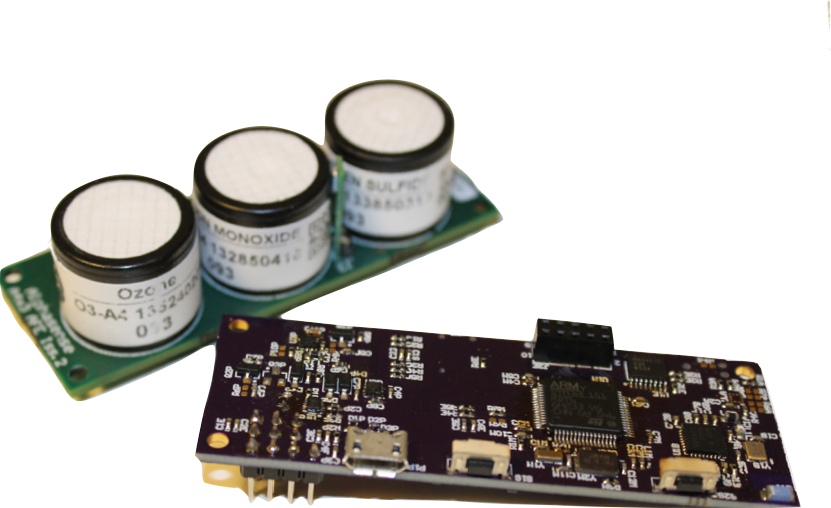
\includegraphics[width=\textwidth]{visuals/learnairV3} \centering              
 	 \caption{Third revision, STM32L152-based learnAir main board next to the AlphaSense sensors}
  	\label{fig:learnairV3}
\end{figure}

\clearpage

\FloatBarrier
\section{Hardware Comparison and Analysis}
\FloatBarrier

MassDEP hardware uses robust, FEM certified techniques-- thus it can be taken as a grounded reference over the time-scales it measures.  The corresponding air quality sensors in the learnAir system are variable in quality, and their analysis is discussed in Chapter 7.    Most of the remaining sensors included in the learnAir system are robust and well-characterized for their purpose.

To validate proper function, in this section we compare temperature and humidity readings from the learnAir device against corresponding weather API data retrieved from ForecastIO for the latitude and longitude of the device.  We also analyze and compare our experimental differential pressure wind sensing design against the ground-truth MassDEP wind speed and wind direction.

ForecastIO data is hourly, and a 60 minute rolling average is used to interpolate the values to the minute timescale.  LearnAir data is collected every minute.

\subsection{Temperature and Humidity}
\FloatBarrier

\begin{marginfigure}[5cm]
 	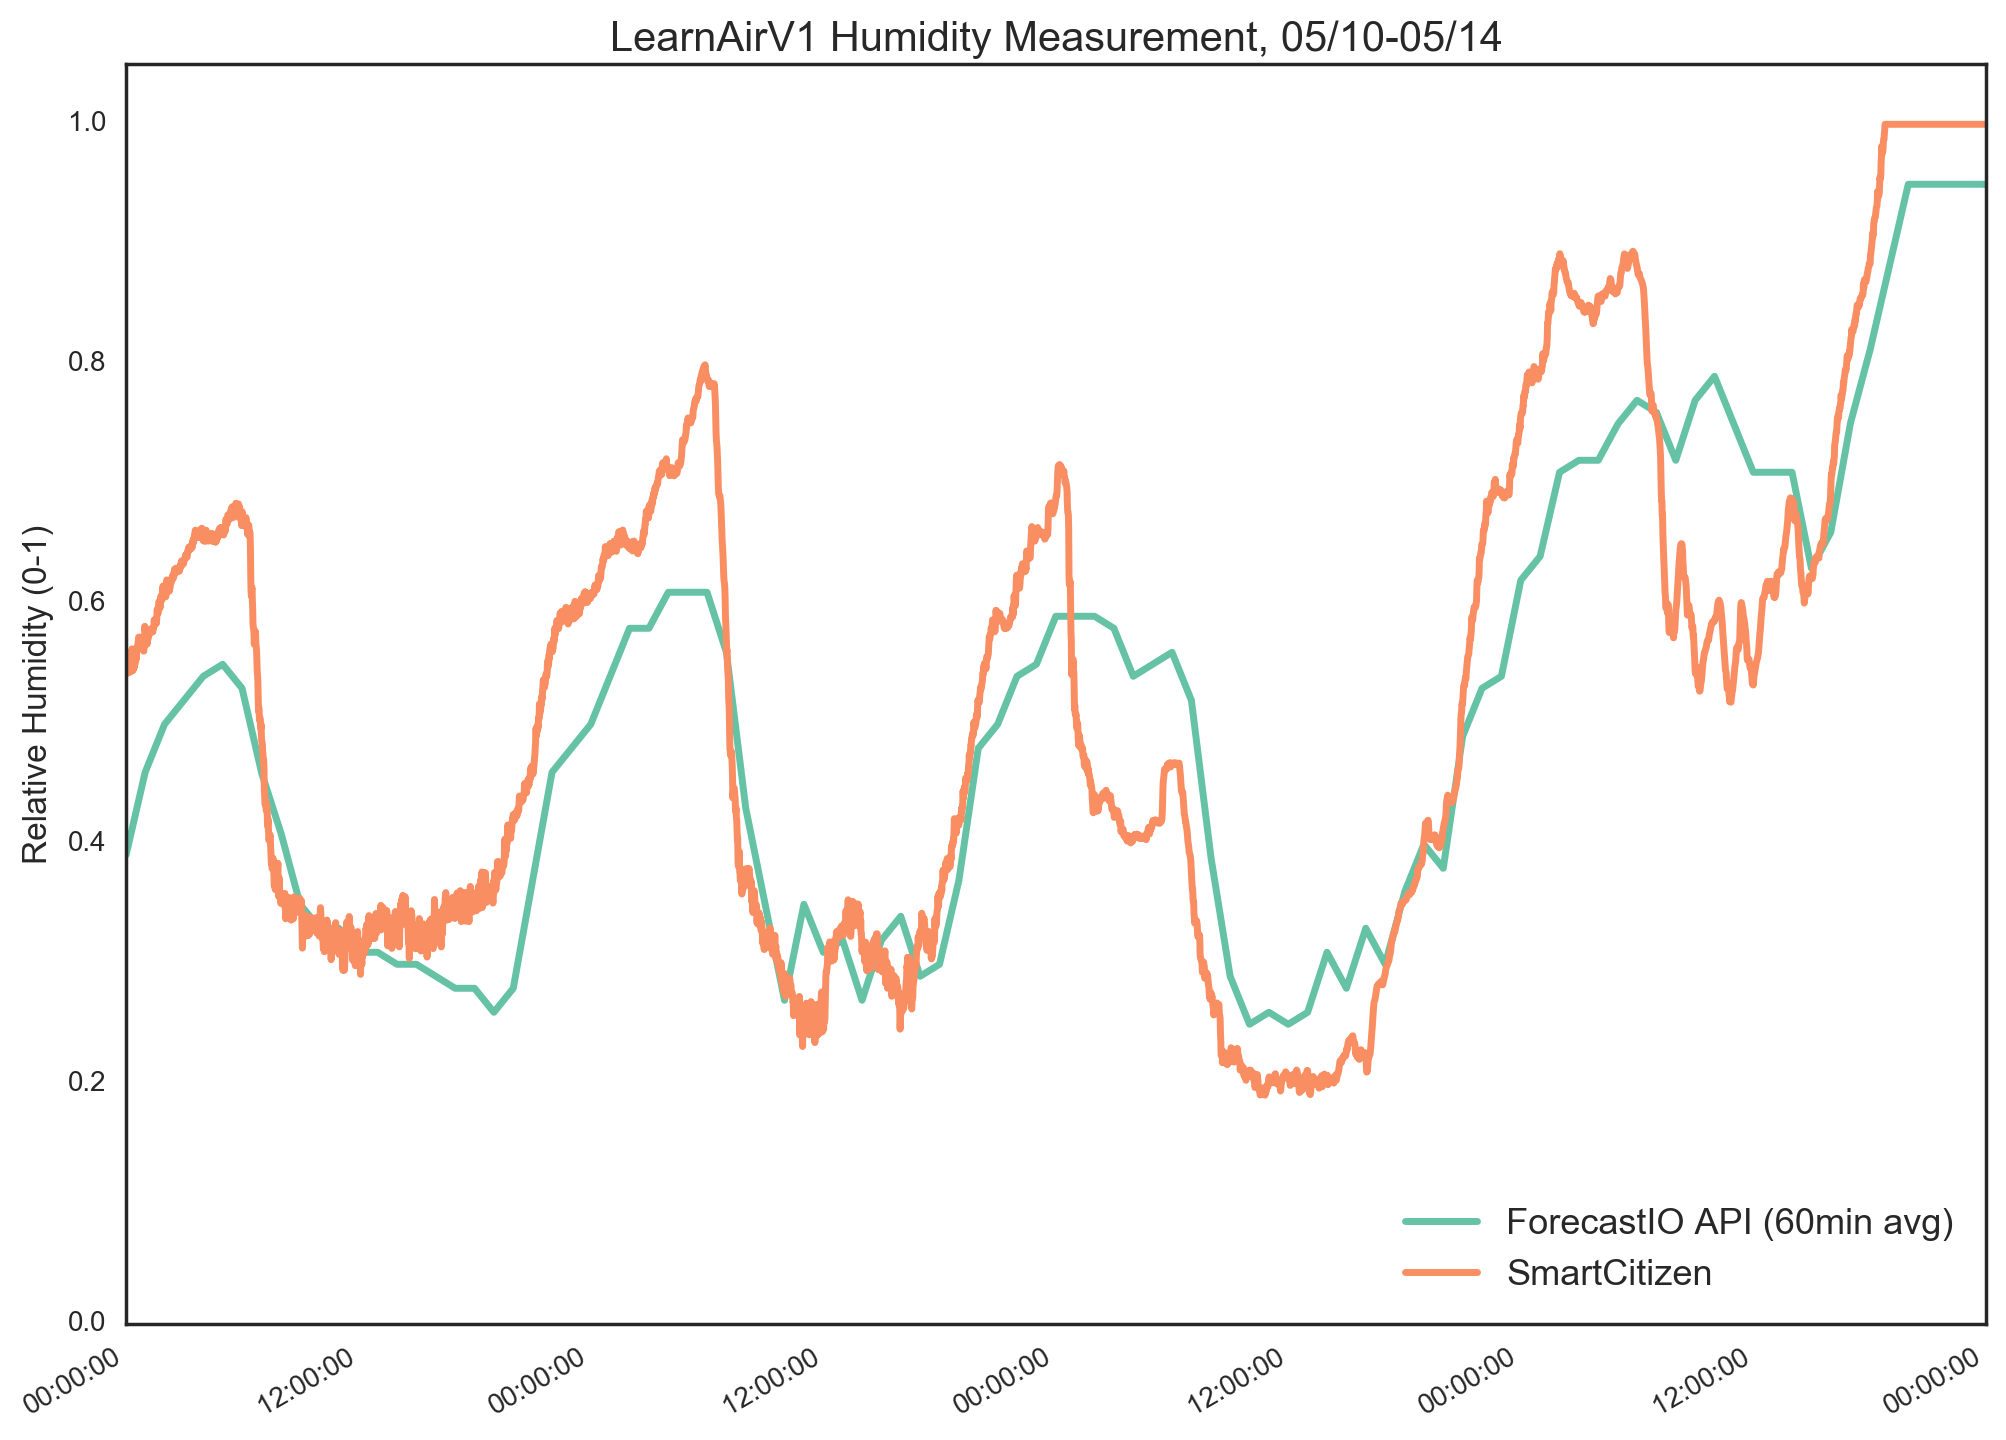
\includegraphics[width=\textwidth]{figs/humidity_zoomed}               
 	 \caption{Humidity Comparison of SmartCitizen (orange) and ForecastIO (green) over 4 days}
  	\label{fig:humidity_zoomed}
\end{marginfigure}

Humidity was recorded in the box by the SmartCitizen Kit and compared against the ForecastIO reading.  Figure \ref{fig:humidity_sck_v_forecastio} shows a comparison of each SmartCitizen reading with each ForecastIO value-- ideally they would track closely, falling on the 1:1 line when plotted against each other.  Instead we see a slight skew towards higher humidity in the box.  It is reasonable to assume this is a real phenomena-- temperature differential in the box may cause condensation and elevated humidity.  In either case, the consistency between the measurements is quite good, and suggests trustworthiness. 

\begin{figure}[htb]
 	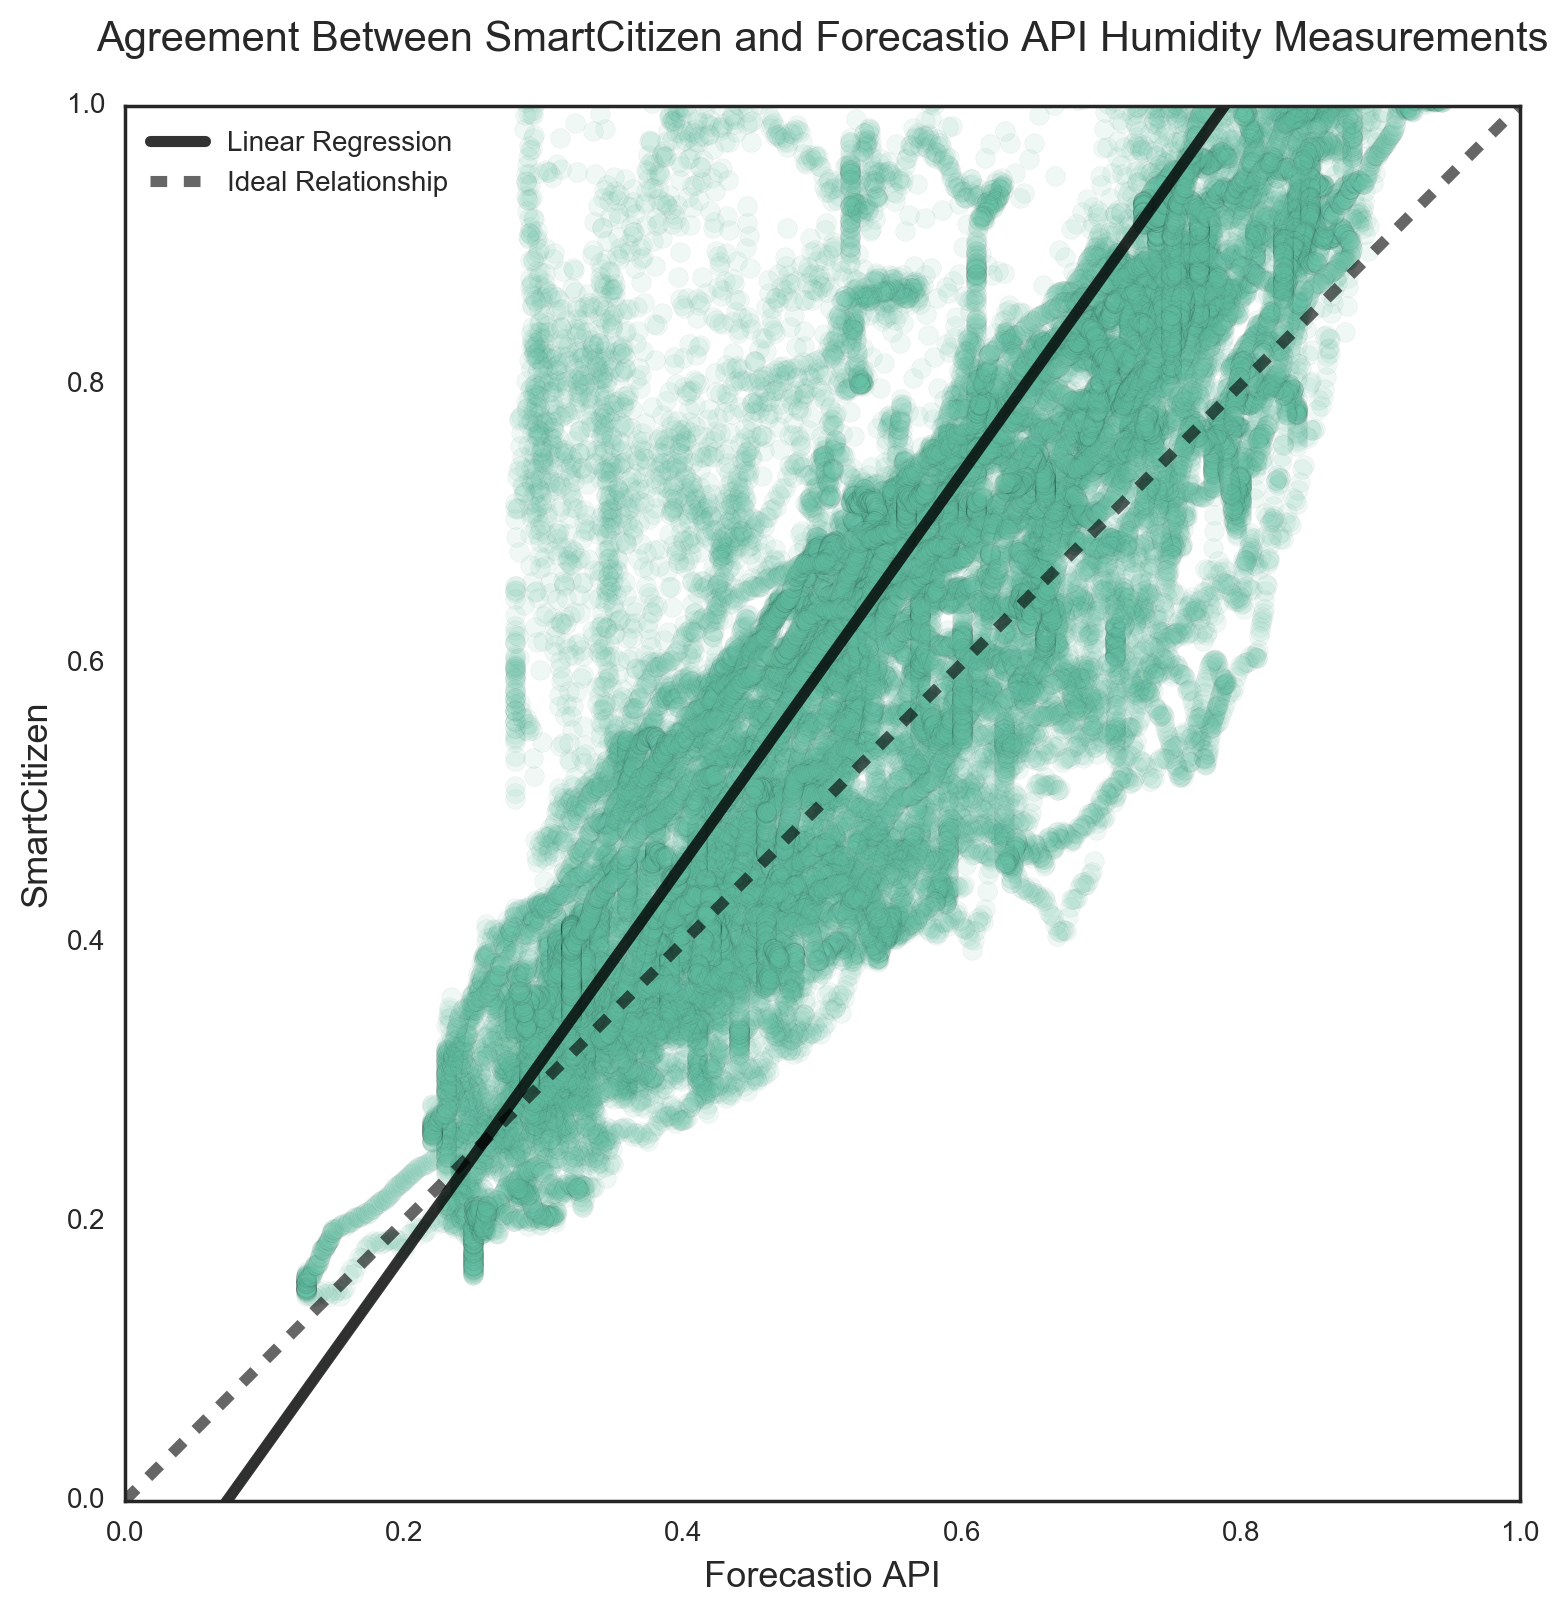
\includegraphics[width=\textwidth]{figs/humidity_sck_v_forecastio}               
 	 \caption{Humidity Comparison, SmartCitizen and ForecastIO}
  	\label{fig:humidity_sck_v_forecastio}
\end{figure}

\begin{marginfigure}[3.5cm]
 	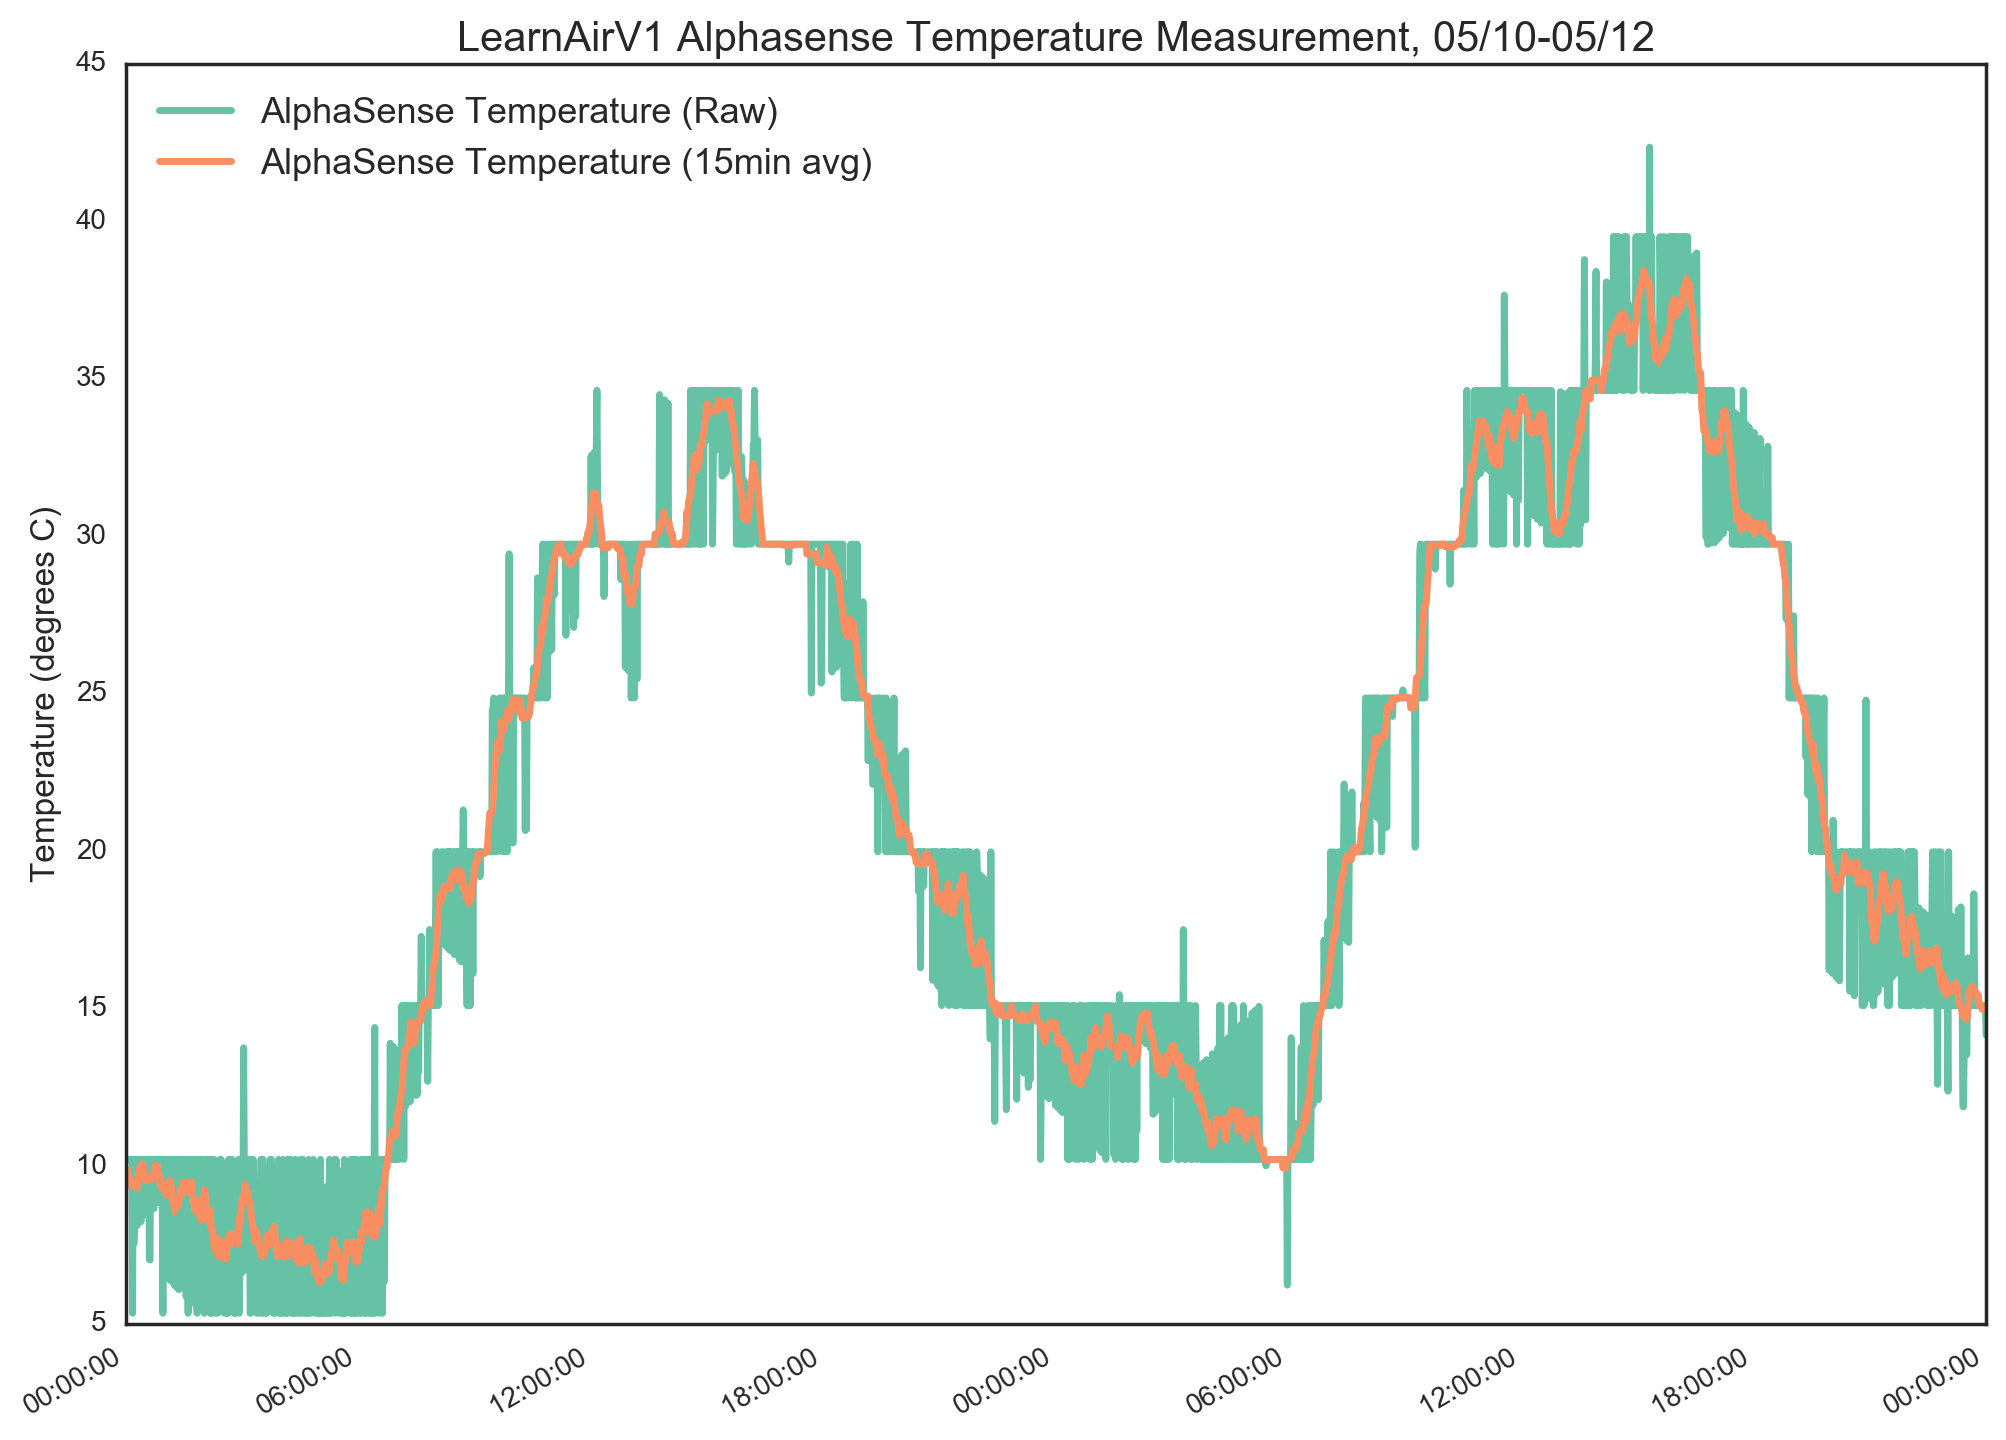
\includegraphics[width=\textwidth]{figs/temp_alphasense}               
 	 \caption{Alphasense Raw Temperature Data (green) with 15-minute averaging (orange)}
  	\label{fig:temp_alphasense}
\end{marginfigure}


Temperature was recorded inside the box by both the AlphaSense temperature sensor and the SmartCitizen Kit.  Figure \ref{fig:temp_alphasense} shows quantization error on the raw AlphaSense reading (teal)-- this is mitigated by taking a 15-minute rolling average (orange).  In Figure \ref{fig:temp_zoomed} we see a four day comparison of ForecastIO data with data taken in the box from the AlphaSense and SmartCitizen sensors.    We see good agreement between in-the-box data, with some slight variation as temperatures exceed 25 degrees Celcius.  There is also good agreement between the ForecastIO data and the in-the-box data when the sun is down.  This is a real effect-- the learnAir box was exposed to direct sunlight, and thus shows significant rises in temperature during the day compared with ambient conditions.  Both temperatures (and their differential) are used to as features for our machine learning algorithm, with in-the-box temperatures informing our calibration process (which is appropriate as the air quality sensors are likewise in the box).   

\begin{figure}[htb]
 	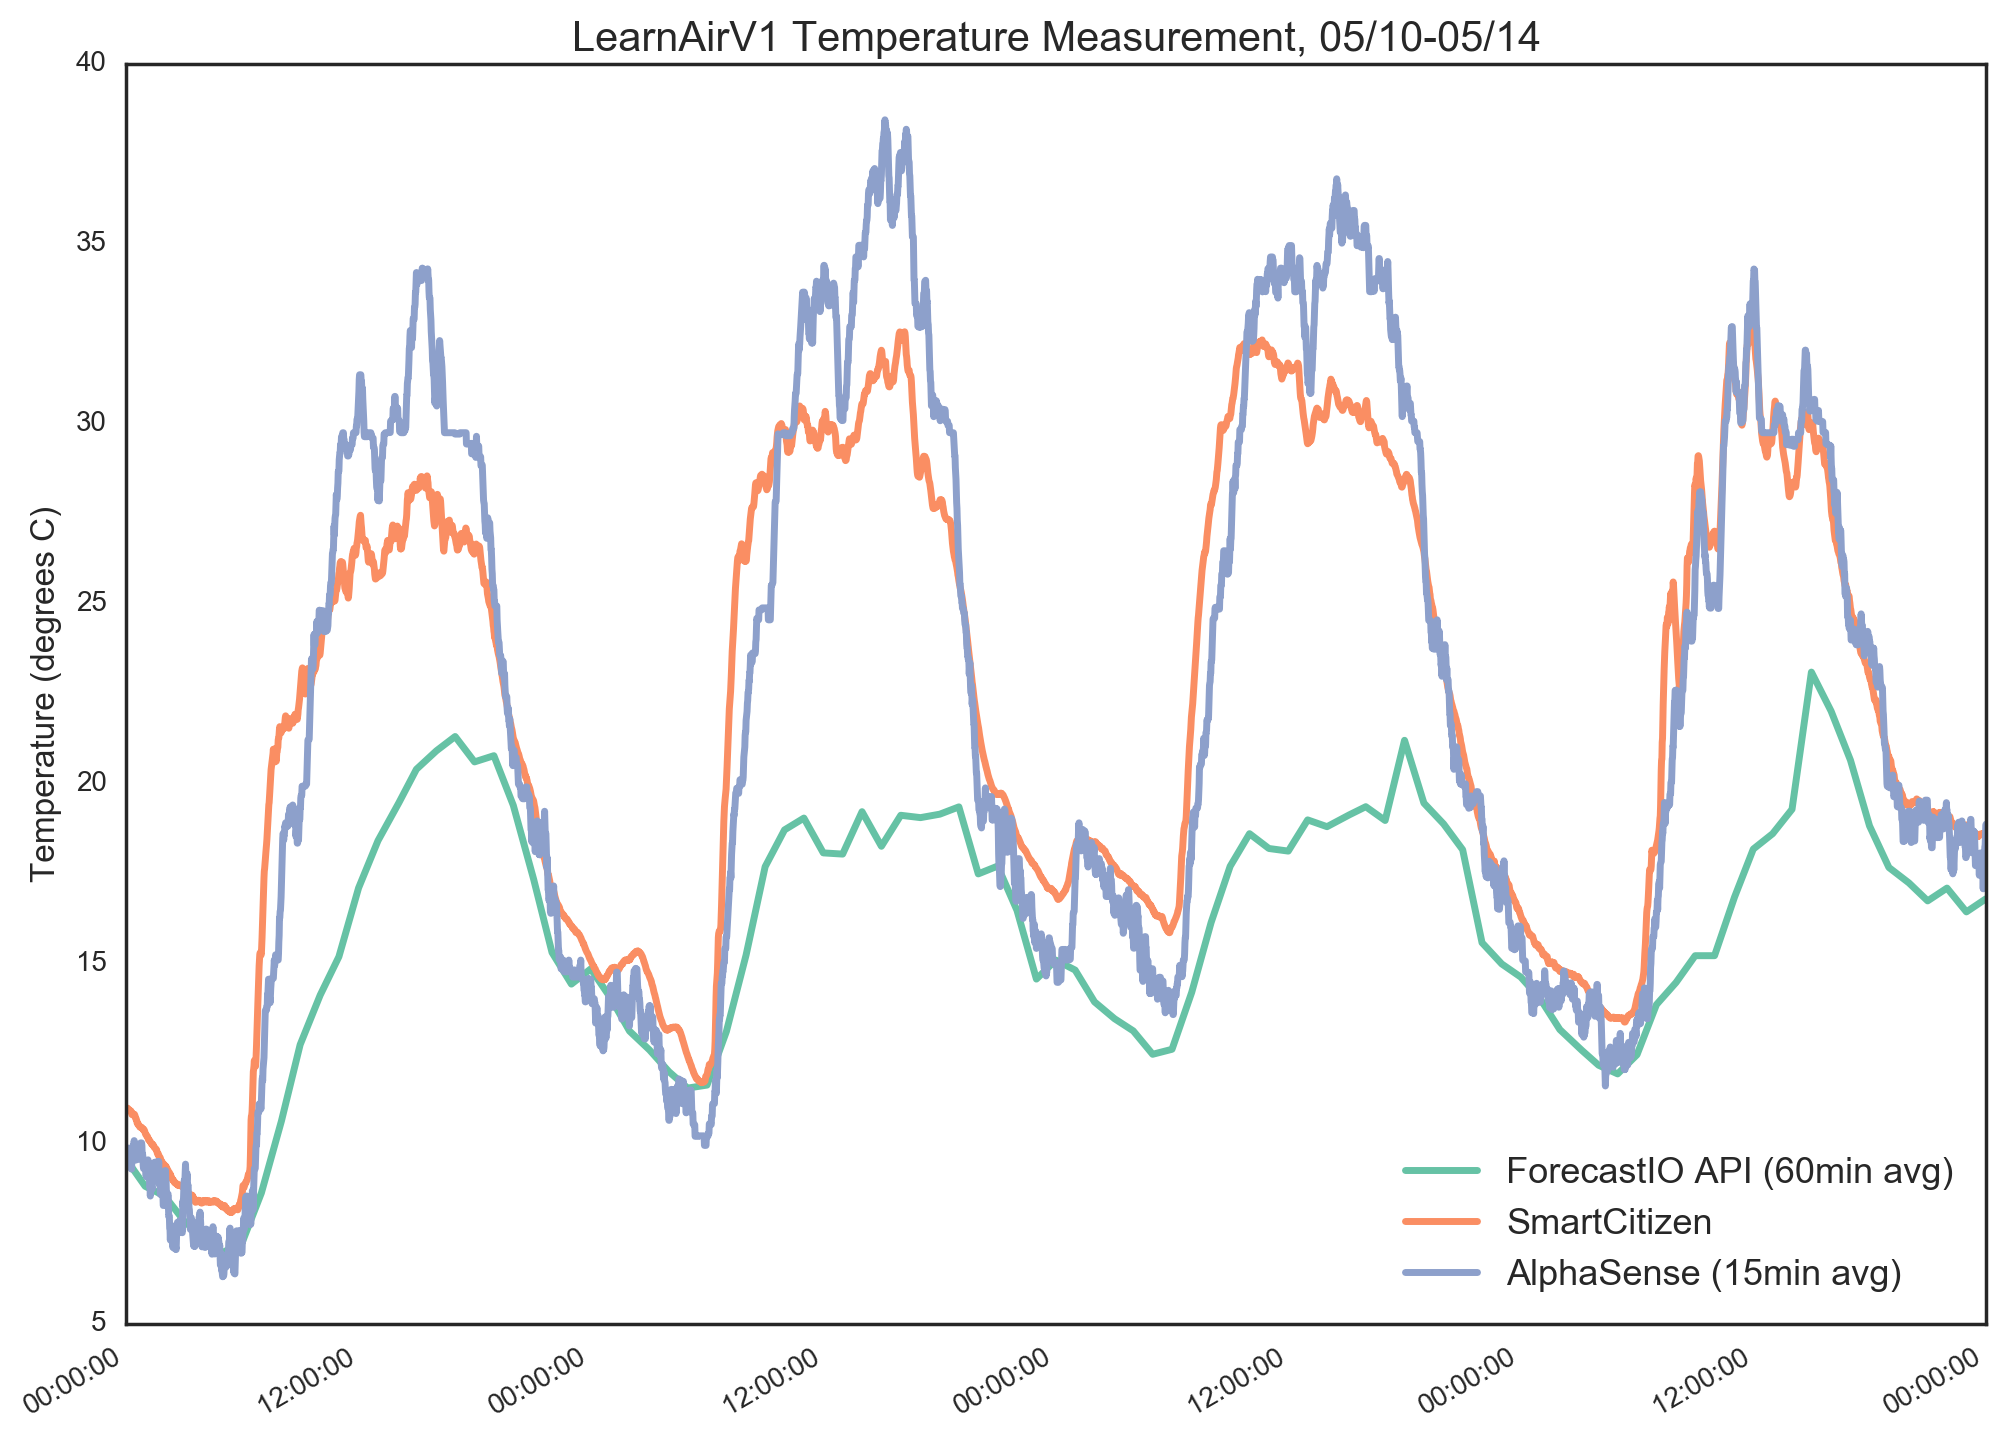
\includegraphics[width=\textwidth]{figs/temp_zoomed}               
 	 \caption{Temperature close-up}
  	\label{fig:temp_zoomed}
\end{figure}

\begin{marginfigure}[3.5cm]
 	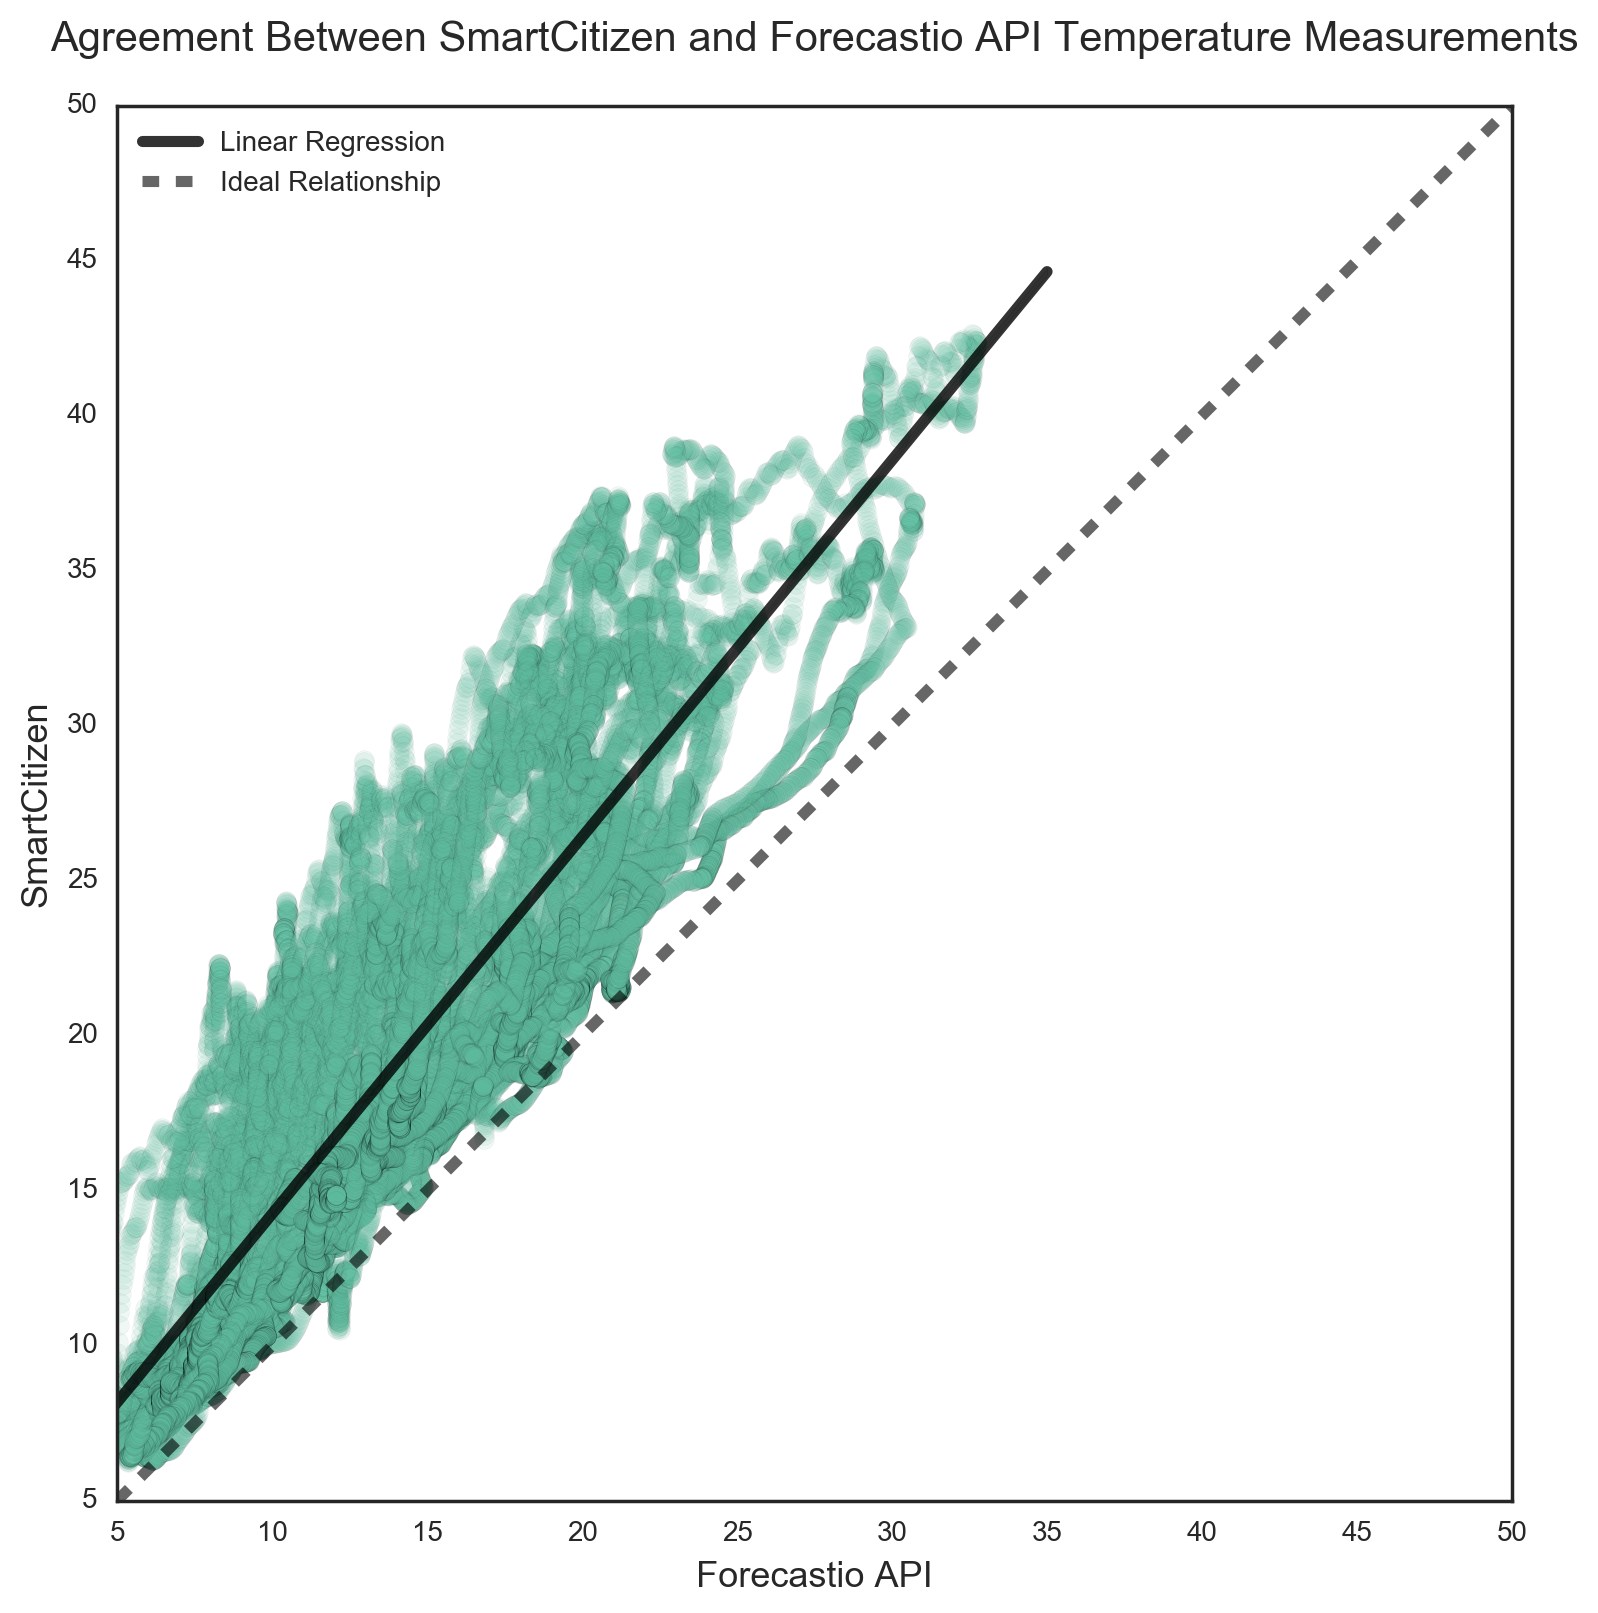
\includegraphics[width=\textwidth]{figs/temp_forecastio_v_sck}               
 	 \caption{Temperature Comparison, SmartCitizen and ForecastIO}
  	\label{fig:temp_forecastio_v_sck}
\end{marginfigure}

\subsection{Wind}
\FloatBarrier

Using differences in pressure to sense wind direction is not a new concept-- pitot tubes (frequently found on airplanes) are one such example.  Recent work to create MEMs wind sensors using this modality has also started to appear. \cite{wind}  It is not typical to find differential pressure sensing used in this way, however; particularly at this scale, and taking into account (or potentially leveraging) the geometry of a larger box.

Thus, the included differential pressure sensor was a small, cheap, and experimental way to measure airflow and wind through the device.  One of its two ports is connected to the side of the box with a tube, while the other is vented into the box-- since the box has holes and is pressure equalized, any differences we measure can be attributed to wind on the outside box face.  While the learnAir V1 sensor only had one differential pressure sensor in it (mounted on the same face as the other sensor inlets), the boards were designed to support three axis sensing, in order to get a truly 3-D understanding of wind speed and directivity and how that may affect air quality measurement.  Doing so accurately requires polar pattern analysis, orthogonality in wind response vs. direction, and some interesting device geometry and signal processing.  This is an open research question in and of itself.  In this first instance, only one axis (measuring speed and not direction) was captured on the primary face of the device.

As a first step to explore the feasibility of such a wind sensing system, the learnAir system was (1) characterized using a home-made laminar flow setup, and then (2) compared against trustworthy external wind speed and direction data from MassDEP.  

The goal of the first test was to get a sense for learnAir's wind direction selectivity.  Since the design is rectangular and the wind sensor is protected by a slotted design, we would expect air flow parallel with the slots to penetrate less than perpendicular flow.  We'd also expect air coming directly at the sensing face of the device to penetrate much more than air flow coming at the back.

\begin{marginfigure}
 	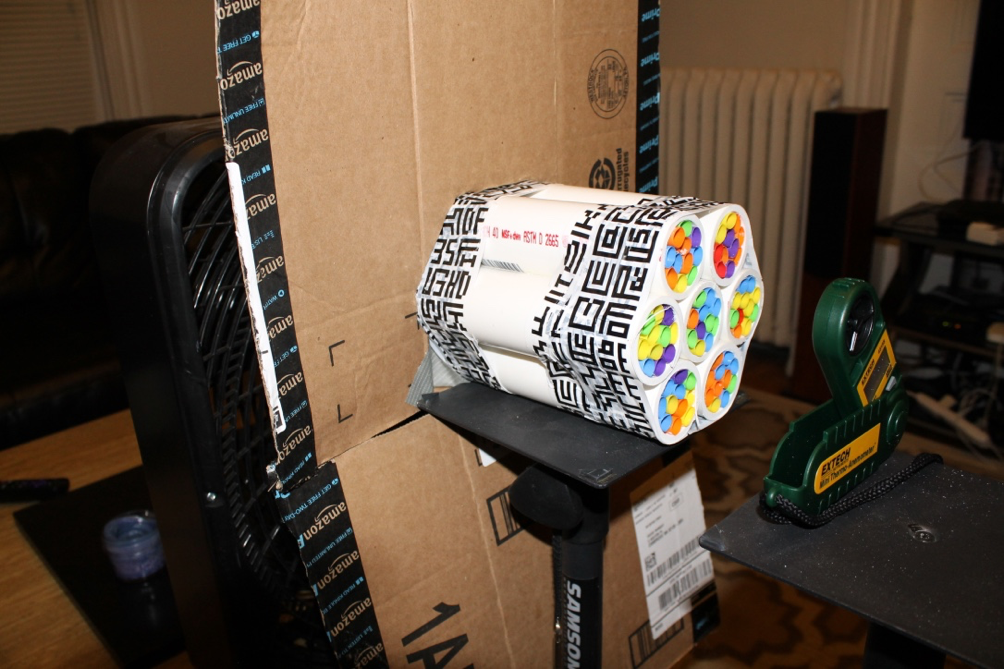
\includegraphics[width=\textwidth]{visuals/windtest}               
 	 \caption{A picture of a simple laminar flow test setup for rough wind directivity characterization}
  	\label{fig:windtest}
\end{marginfigure}

\enlargethispage{2cm}


To test this, PVC pipes filled with large straws was placed in front of a fan to approximate laminar flow conditions (Figure \ref{fig:windtest}).  Cardboard was placed around the laminar flow section to prevent spurious eddy currents.  A handheld Extech 45158 Anemometer was used to validate a constant airflow of 2 m/s (a light breeze).  The learnAir V1 device was then placed in the flow, and rotated at 30 degree intervals, with 10 wind measurements at each interval.  The top half of figure \ref{fig:wind_polar} shows a normalized polar response with air flowing directly towards the slotted wind sensor device face at 0 degrees (and directly at the rear face of the device at 180).  The bottom half shows the response of the device with wind flowing over top of the face at various angles-- 0 degrees represents airflow parallel with the short dimension of the learnAir box, and 90 degrees is parallel with the long dimension.

\begin{figure}[htb]
 	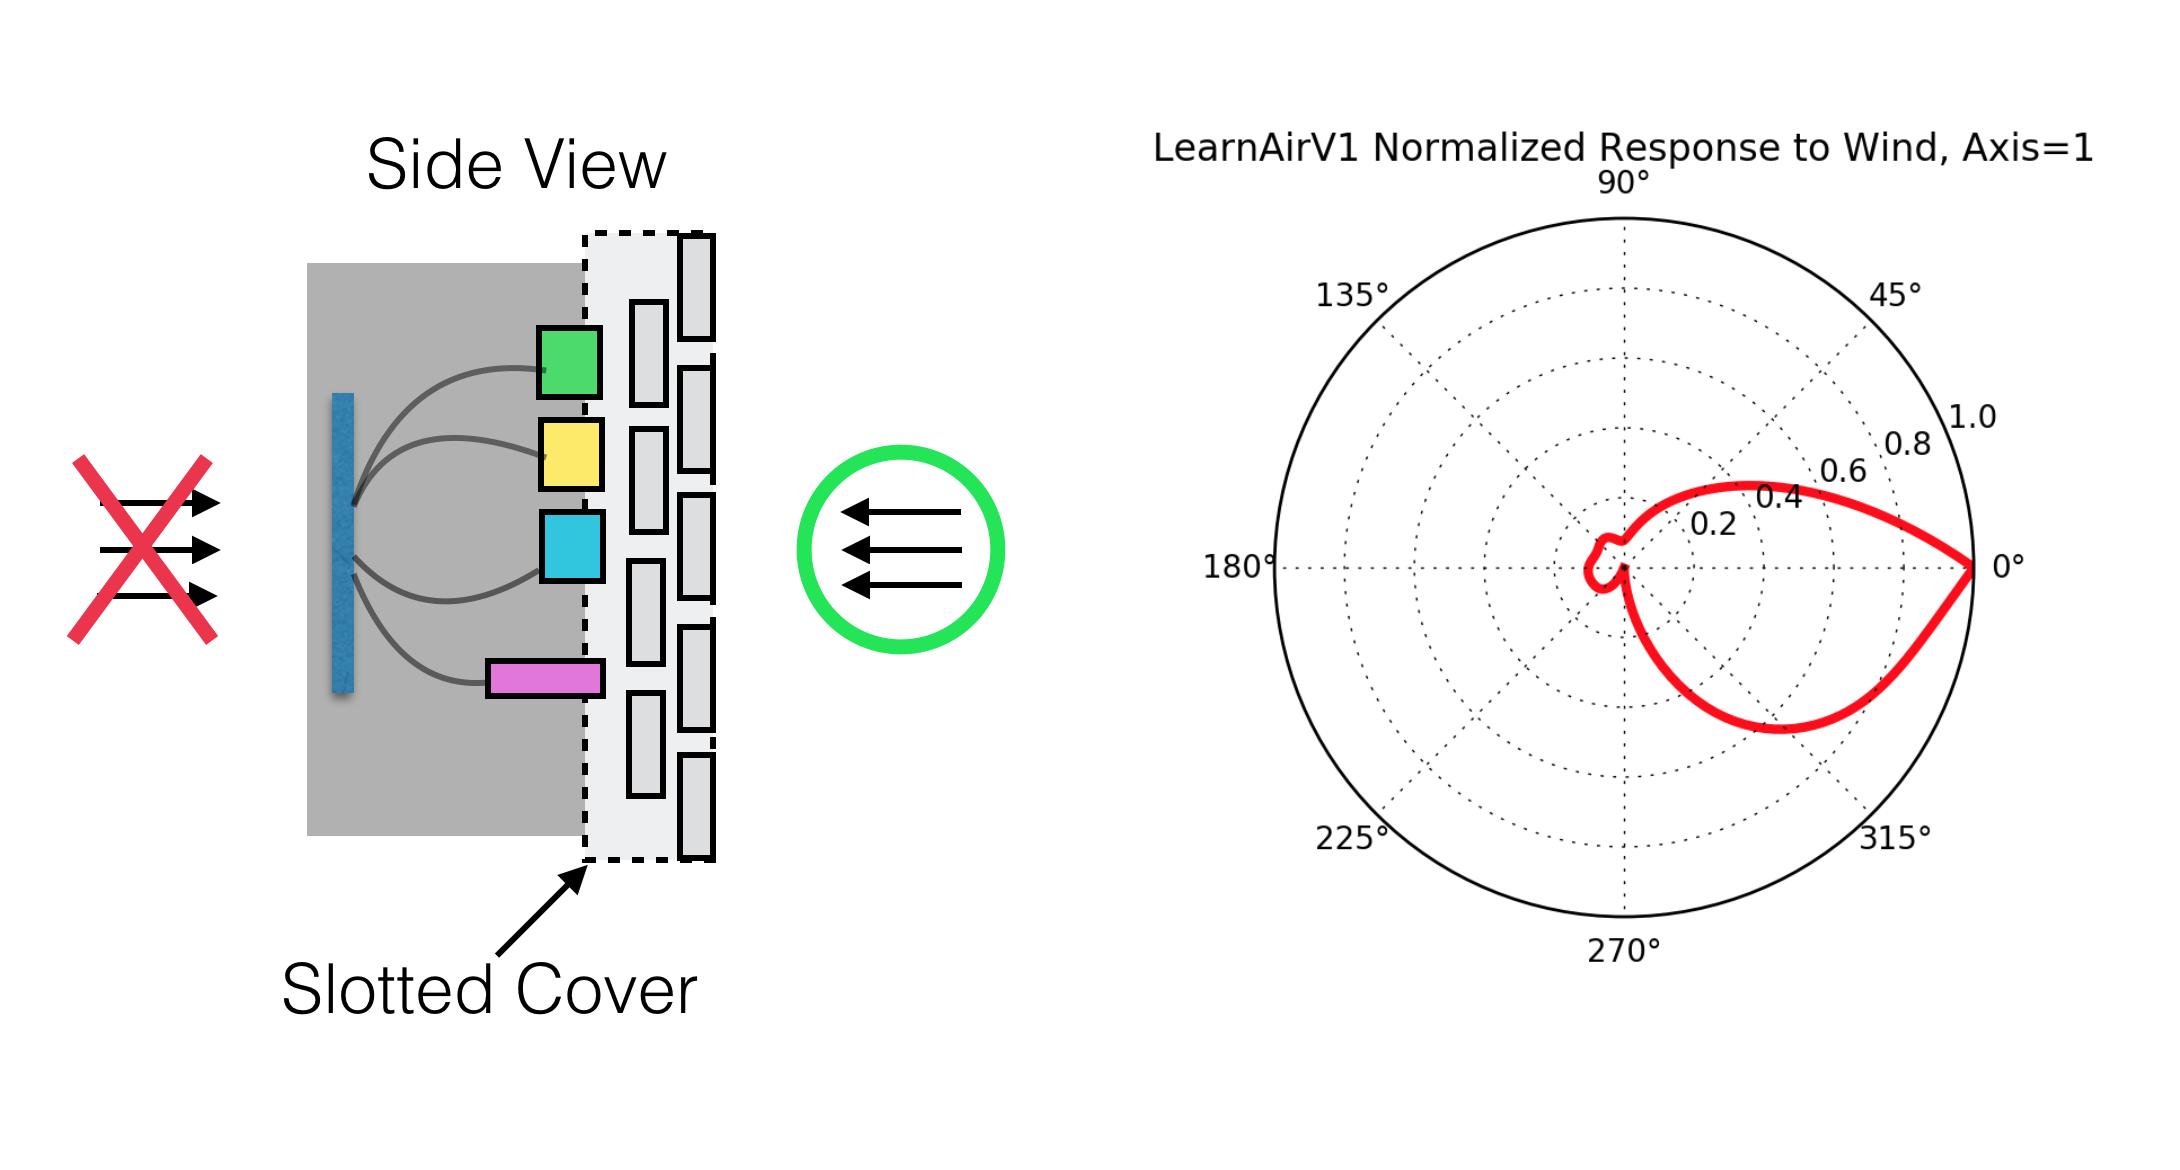
\includegraphics[width=\textwidth]{figs/wind_polar_1}               
 	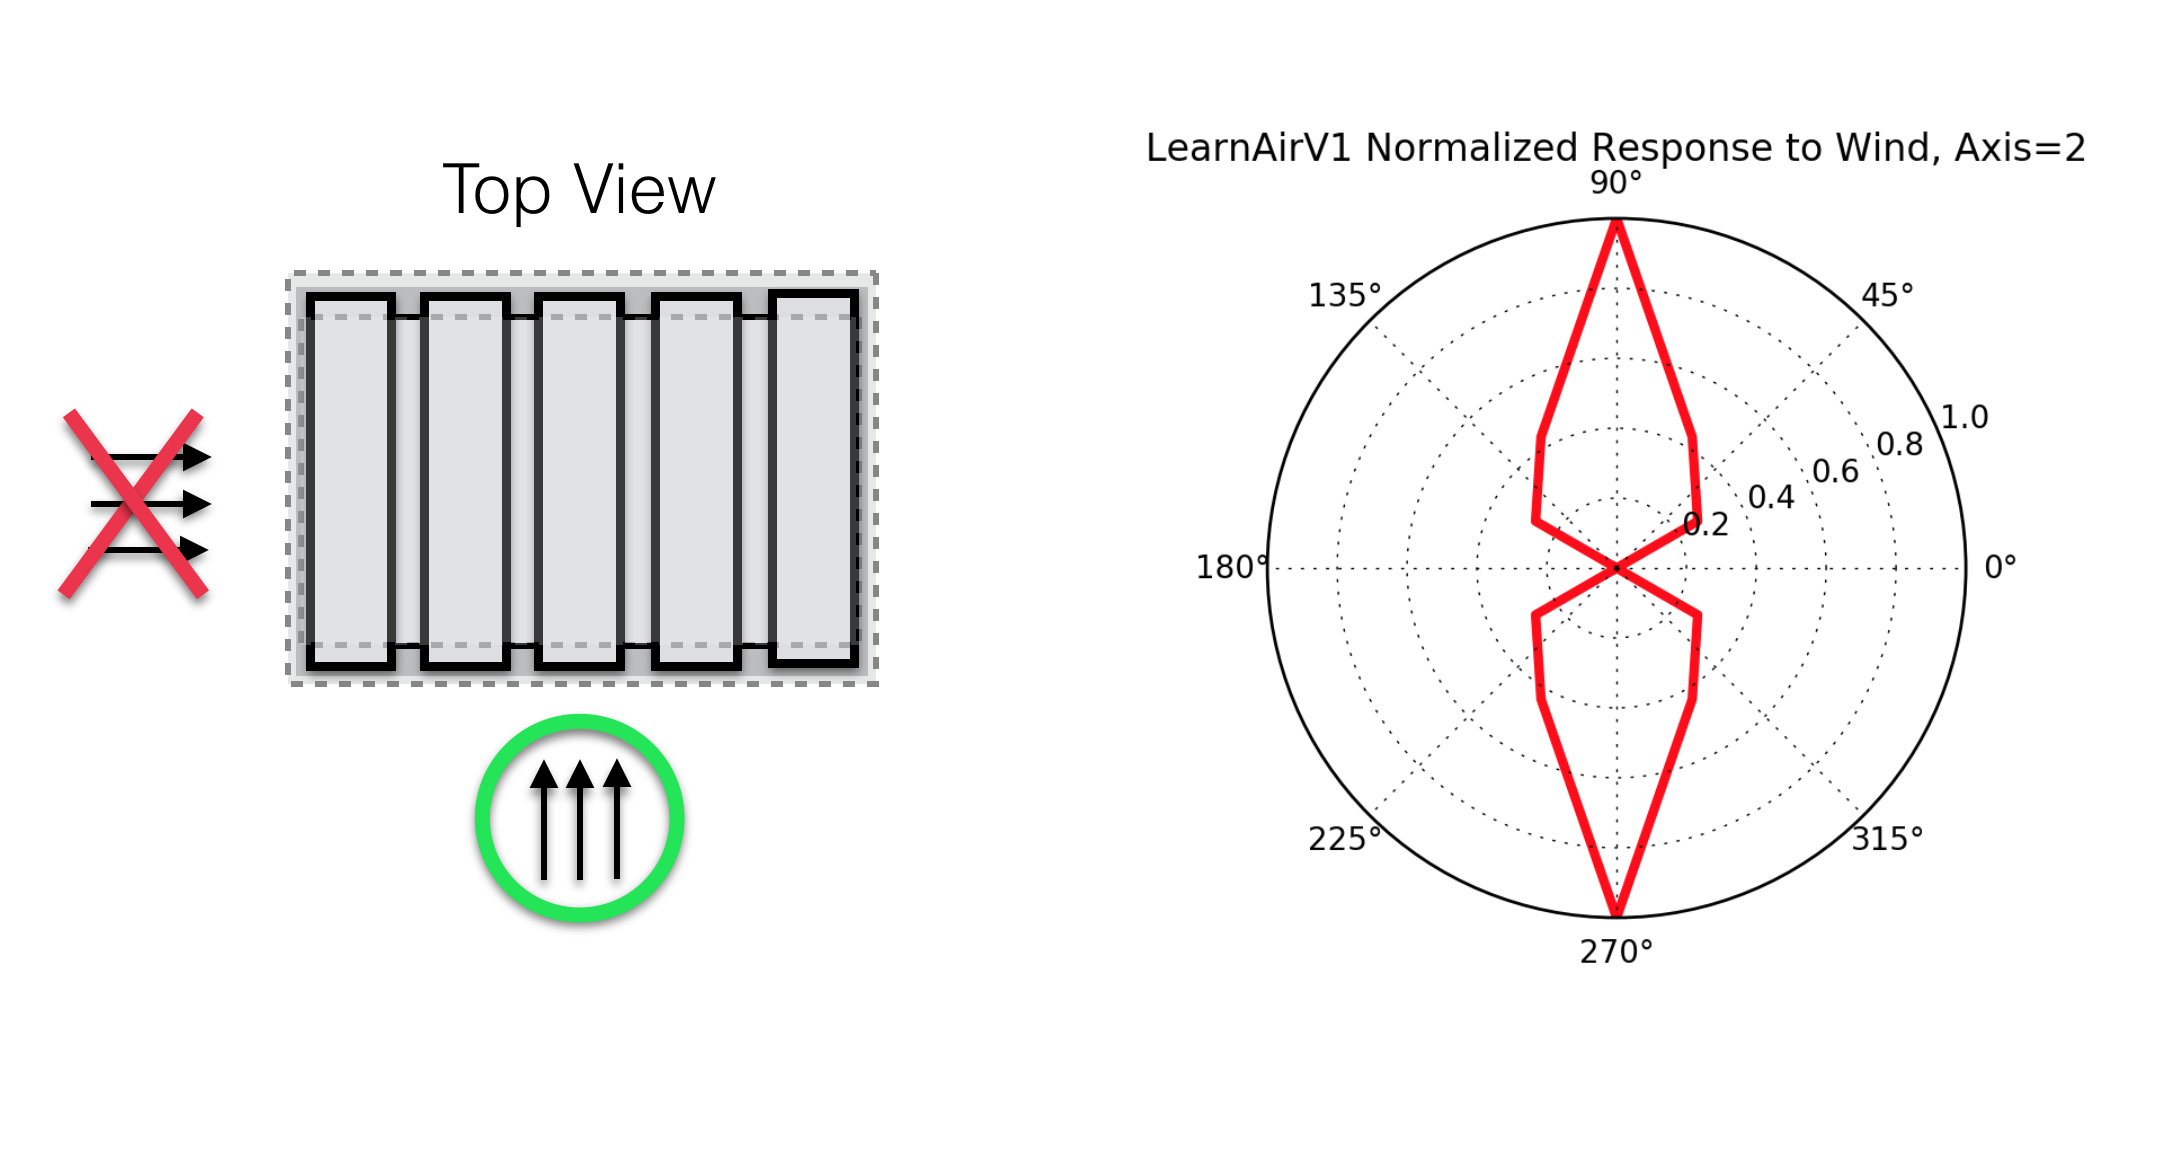
\includegraphics[width=\textwidth]{figs/wind_polar_2}               
 	 \caption{Wind Directivity Polar Patterns}
  	\label{fig:wind_polar}
\end{figure}

As expected, the device responds with an interesting 3 dimensional pattern.  It is very responsive to airflow coming at the face, and very insensitive to air flow coming from behind.  It is very sensitive to airflow perpendicular to its slots, and completely insensitive to airflow that is parallel.  This is a very useful feature to exploit for truly three dimensional wind sensing, and for controlling device airflow.  Designs that include checkerboard slots or slots in both directions may be very impervious to wind.  At the same time, with no active airflow through the device, these results suggest that the air that is being sampled is (1) more likely to be pushed into the cavity from specific directions, which may artificially affect how sensitive to directional sources of pollutions like a nearby road, and (2) we may expect some low-pass filtering effects relative to a sensor design that actively pulls air through the device, especially when the wind is blowing in a direction that has difficulty penetrating the slotted cover. 

\pagebreak

The second test compares windspeed measured by the device with windspeed measured externally by the MassDEP sensor.  We would expect, given our polar plots, that (1) the actual airflow we're sensing is different/shielded from the real wind, so there may be some differences in the measurement, and (2) our device is selective to certain wind directions, so it is important to analyze the relationship of errors in our readings compared with the MassDEP readings as a function of wind direction. 

Figure \ref{fig:ws_with_10_accuracy_zoomed} shows a comparison of measured windspeed data from our pressure sensor against the MassDEP data for one day (after pre-conditioning the signal and LMSE scaling it against the MassDEP reference).  There is a clear correlation in overall trend, suggesting the pressure sensor is capturing meaningful information.  Tight agreement of $\pm$5\% between readings is highlighted in green.   

\begin{figure}[htb]
 	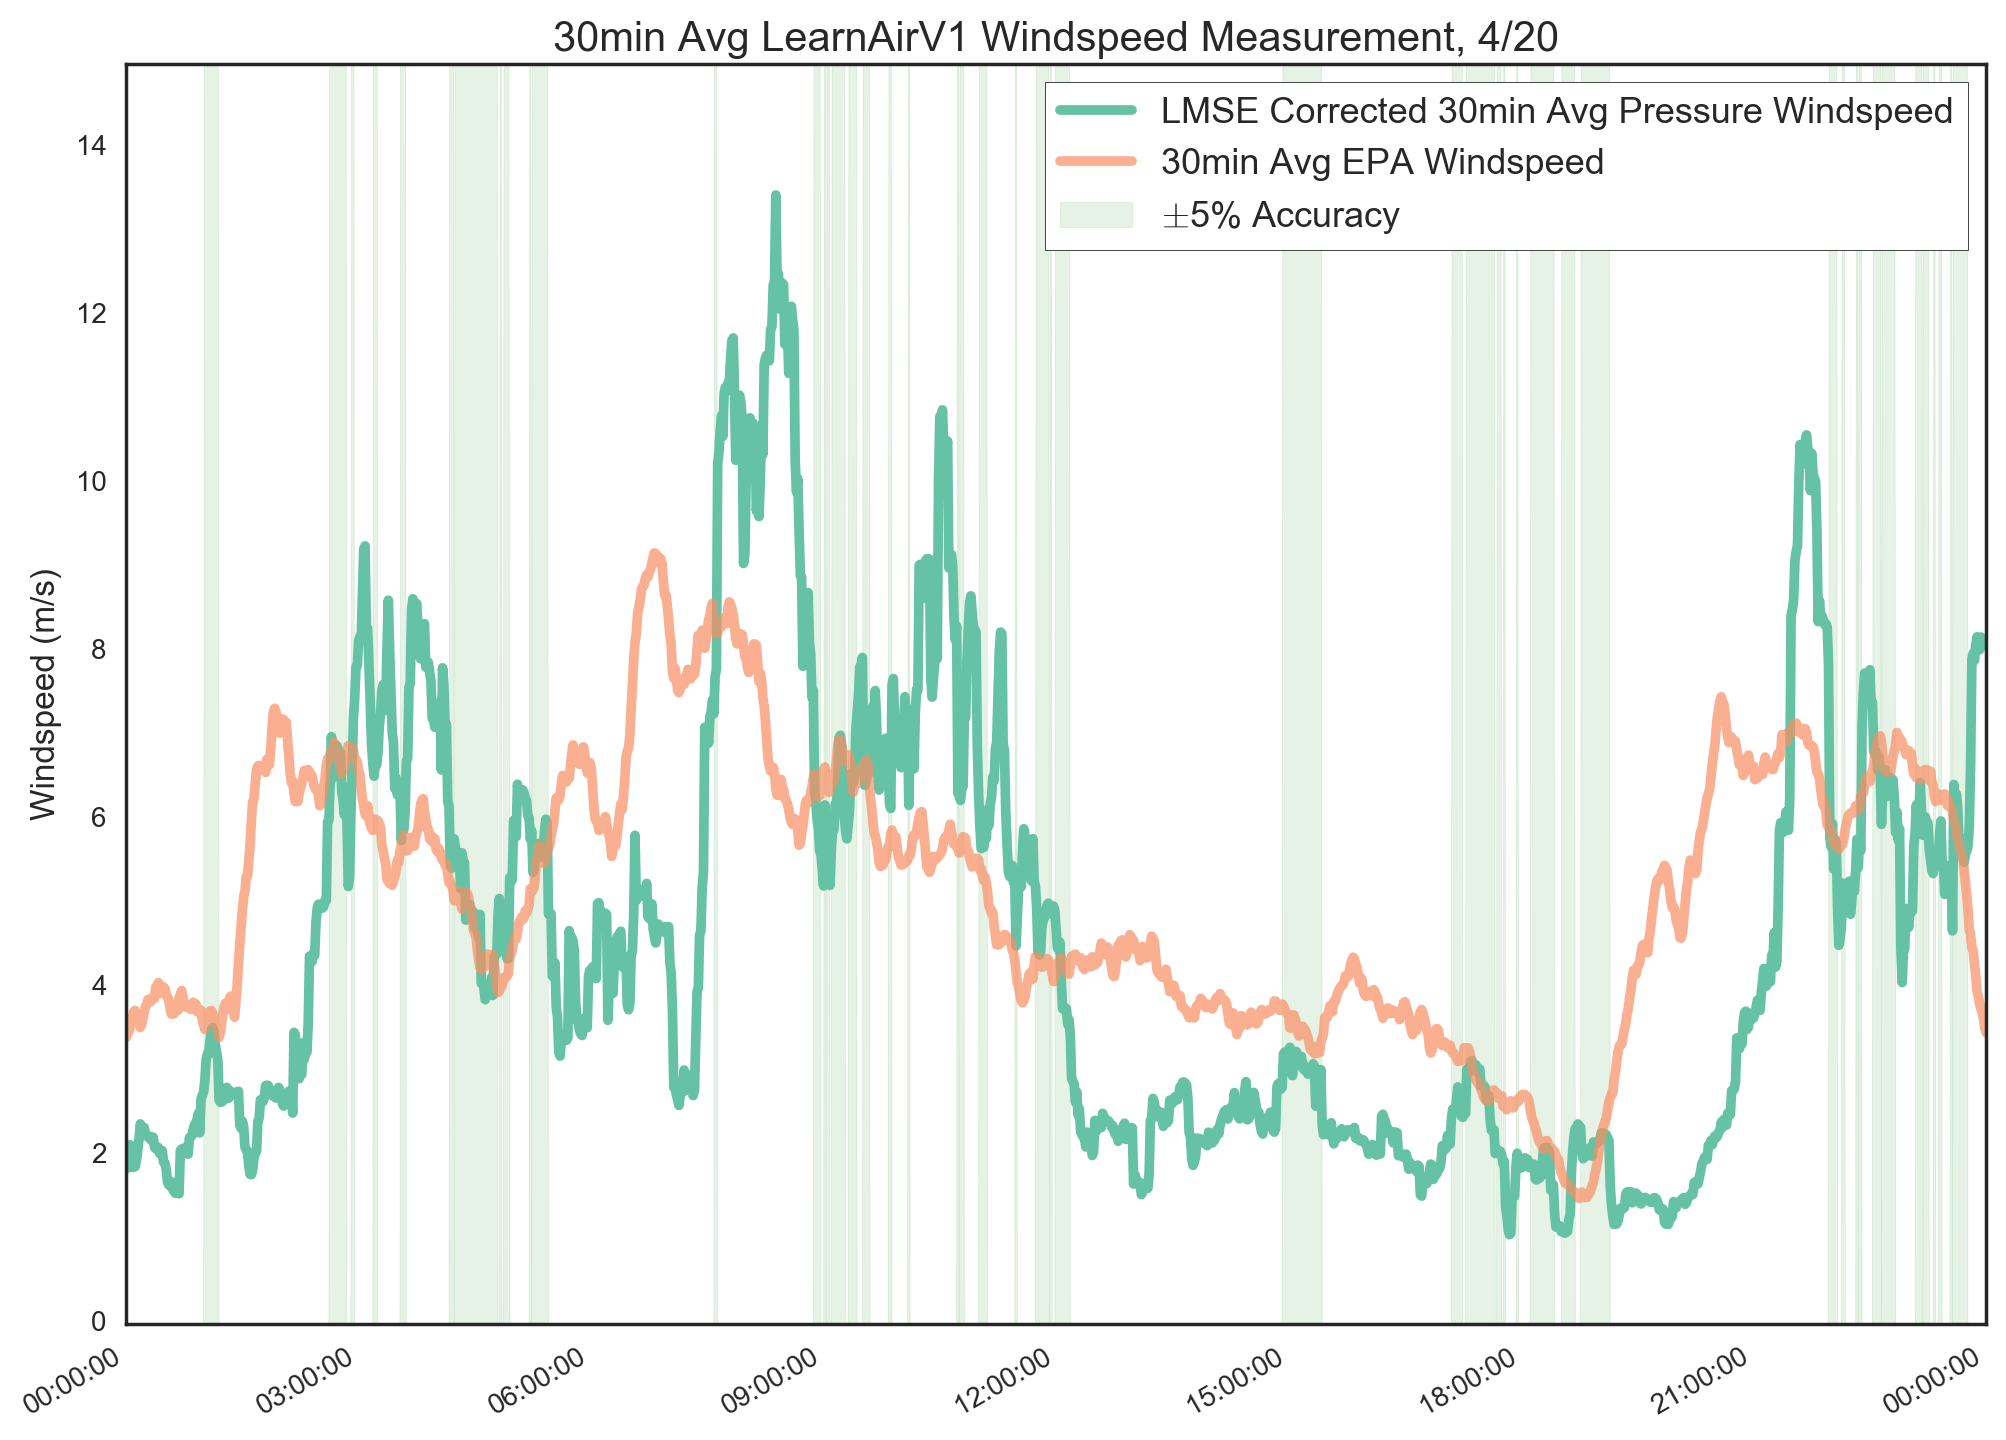
\includegraphics[width=\textwidth]{figs/ws_with_10_accuracy_zoomed}               
 	 \caption{Wind Speed Measurement with 10\% Accuracy, Zoomed}
  	\label{fig:ws_with_10_accuracy_zoomed}
\end{figure}

While the overall trend is there, there are some large discrepancies.  Based on our polar plots, it seems worthwhile to look at the differences between our measurement and the MassDEP measurement as a function of wind direction, as shown in Figure \ref{fig:ws_error_vs_wd}.  There are clear and interesting relationships between measurement inaccuracies and wind direction-- there are large differences in the readings when the wind approaches from ~60, 120, 210, 270 degrees, while 0, 90, 180, 260, and 320 degrees seem to match more closely.  This does not corroborate expectations exactly, given our polar plots (0 and 180 degrees having low error since they allow wind to pass, and 90 and 270 degrees having high error since they reject airflow).  These results suggest a more complicated relationship between direction and selectivity.  More rigorous testing is required to accurately characterize the directionality of this system.

\begin{figure}[htb]
 	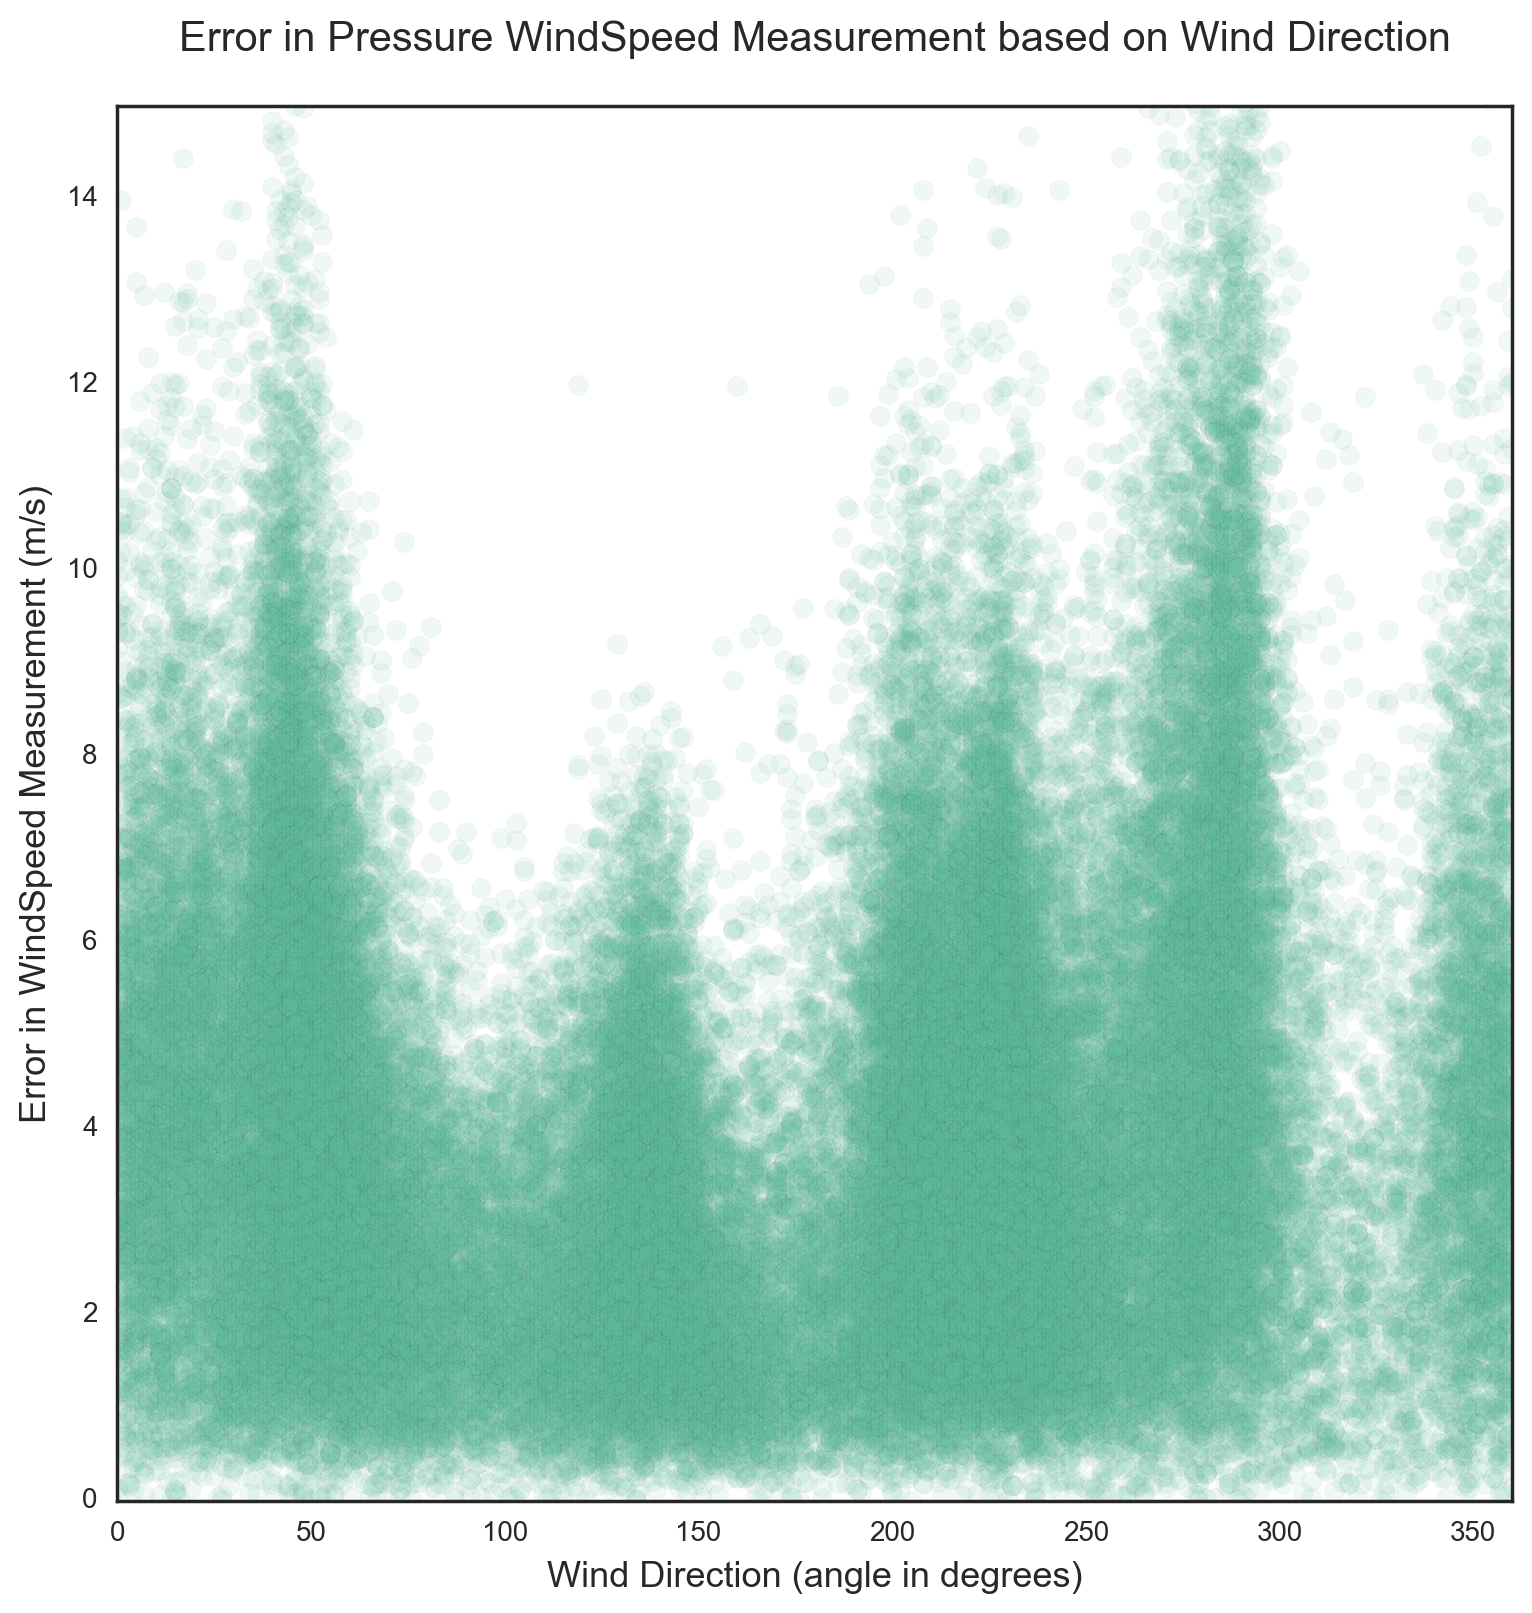
\includegraphics[width=\textwidth]{figs/ws_error_vs_wd}               
 	 \caption{Discrepency in Windspeed Measurement vs Wind Direction}
  	\label{fig:ws_error_vs_wd}
\end{figure}

The overall trends support the fact that our pressure sensor is measuring airflow in a correct and useful way.  Having a measure of airflow inside the slotted casing is good for tracking meaningful penetration of wind, regardless of direction.  This work suggests that pressure sensors have great potential to provide a low cost, small option for accurate wind sensing.  Future research is necessary to optimize sensor geometry, orthogonalize sensor axes, and characterize the effect of device geometry and turbulence on system linearity, in order to understand the wind sensing potential for this technology.  For this project, the pressure signal provides insight regarding near-field air flow that can be used as a training feature for our machine learning model.  More figures describing the wind data can be found in the Appendix.
